%% ------------------------------------------------------------------------ %%
% GJI ARTICLE MODE
%% ------------------------------------------------------------------------ %%
\documentclass[referee,extra]{gji}
%\documentclass[extra,mreferee]{gji}
%%%%% older
%\documentclass[11pt,extra]{gji}

%\documentclass[referee,extra]{gji} % galley/ referee
\usepackage{appendix}

%%%%\usepackage{timet}
\usepackage{graphicx}
\usepackage{amsmath}
\usepackage[dvipsnames,usenames]{color}
\usepackage[colorlinks=true,citecolor=black,linkcolor=black,urlcolor=blue]{hyperref}
\usepackage{amssymb} % for mathfrak font

%% useful commands
\newcommand{\bequ}{\begin{equation} }
\newcommand{\eequ}{\end{equation} }
\newcommand{\barr}{\begin{eqnarray} }
\newcommand{\earr}{\end{eqnarray} }

\newcommand{\bsplitequ}{\begin{split} }
\newcommand{\esplitequ}{\end{split} }

\newcommand{\oneoverrho}{\frac{1}{\rho} \,  }
\newcommand{\oneoverkappa}{\frac{1}{\kappa} \, }
\newcommand{\intOmega}{\int_\Omega \, }
\newcommand{\intSurface}{\int_{\partial \Omega}}

\newcommand{\bnabla}{ \, {\bf \nabla } }
\newcommand{\bnablaparallel}{ \bnabla^{\|} }

\newcommand{\bs}{ {\bf s } }
\newcommand{\bc}{ {\bf c } }
\newcommand{\bT}{ {\bf T } }
\newcommand{\bforce}{ {\bf f } }
\newcommand{\bM}{ {\bf M } }
\newcommand{\bI}{ {\bf I } }
\newcommand{\bm}{ {\bf m } }
\newcommand{\bx}{ {\bf x } }
\newcommand{\bw}{ {\bf w } }
\newcommand{\bu}{ {\bf u } }
\newcommand{\bv}{ {\bf v } }
\newcommand{\bxi}{ {\bf \xi} }
\newcommand{\bnormal}{ \hat{ \bf{n} } \, }
\newcommand{\bD}{ {\bf D } }

\newcommand{\testw}{ {\rm w } \, }
\newcommand{\tilden}{ \tilde{n} }
\newcommand{\dndntilde}{\frac{\partial_n}{\partial_{\tilden}} }
\newcommand{\abg}{ {\alpha \beta \gamma} }
\newcommand{\aprime}{ {\alpha^{\prime}} }
\newcommand{\bprime}{ {\beta^{\prime}} }
\newcommand{\gprime}{ {\gamma^{\prime}} }

\newcommand{\phionedot }{\dot{ \widetilde{\phi_1} } }
\newcommand{\phioneddot }{\ddot{ \widetilde{\phi_1} } }
\newcommand{\phitwodot }{\dot{ \widetilde{\phi_2} } }
\newcommand{\phitwoddot }{\ddot{ \widetilde{\phi_2} } }
\newcommand{\phithreedot }{\dot{ \widetilde{\phi_3} } }
\newcommand{\phithreeddot }{\ddot{ \widetilde{\phi_3} } }
\newcommand{\phifourdot }{\dot{ \phi_4} }
\newcommand{\phifourddot }{\ddot{ \phi_4 } }

\newcommand{\etal}{ {\it et al. } }
%% biblio GJI
\bibliographystyle{gji}
\renewcommand{\cite}[1]{\citet{#1}}
%% colors to show the corrections
\newcommand{\red}[1]{\textbf{\textcolor{Red}{#1}}}
\newcommand{\blue}[1]{\textbf{\textcolor{Blue}{#1}}}
\newcommand{\cyan}[1]{\textbf{\textcolor{Cyan}{#1}}}
\newcommand{\green}[1]{\textbf{\textcolor{Green}{#1}}}
\newcommand{\magenta}[1]{\textbf{\textcolor{Magenta}{#1}}}
\newcommand{\orange}[1]{\textbf{\textcolor{Orange}{#1}}}
%\newcommand{\red}[1]{#1}
%\newcommand{\blue}[1]{#1}
%\newcommand{\cyan}[1]{#1}

%%%%%%%%%% DK DK
% comments between authors
\newcommand{\todaniel}[1]{\textbf{\red{*** To Daniel, from Dimitri: #1 ***}}}
%\newcommand{\todimi}[1]{\textbf{\magenta{*** To Dimitri, from myself: #1 ***}}}
\newcommand{\fromdimi}[1]{\textbf{\magenta{*** From Dimitri: #1 ***}}}
%%%%%%%%%% RM RM
% comments between authors
\newcommand{\rolandtodaniel}[1]{\textbf{\blue{*** To Daniel, from Roland: #1 ***}}}

\begin{document}

% Uncomment the following code (as well as \usepackage{graphicx} above)
% if you need to include images in draft mode
%%%%%\setkeys{Gin}{draft=false}

%% ------------------------------------------------------------------------ %%
%  AUTHORS
%% ------------------------------------------------------------------------ %%
% Author address will appear at end of article, may repeat
% this command for each author.

\author[Peter et al.]{
\parbox[t]{1.\textwidth}{
Daniel Peter$^1$,
Dimitri Komatitsch$^{2,3}$,
Yang Luo$^1$,
Roland Martin$^2$,
Nicolas Le Goff$^2$,
Emanuele Casarotti$^4$,
Pieyre Le Loher$^2$,
Federica Magnoni$^4$,
Qinya Liu$^5$,
C\'eline Blitz$^2$,
Tarje Nissen-Meyer$^6$,
Piero Basini$^{6}$
and Jeroen Tromp$^{1,7}$
\vspace{1cm}
\newline
{\small
$^1$ Princeton University, Department of Geosciences, 318 Guyot Hall, Princeton, NJ 08544, USA \newline
$^2$ Universit\'e de Pau et des Pays de l'Adour, CNRS \& INRIA Magique-3D,
Laboratoire de Mod\'elisation et d'Imagerie en G\'eosciences UMR 5212,
Avenue de l'Universit\'e, 64013 Pau Cedex, France \newline
$^3$ Institut universitaire de France, 103 boulevard Saint-Michel, 75005 Paris, France \newline
$^4$ Istituto Nazionale di Geofisica e Vulcanologia, Via di Vigna Murata 605, 00143, Rome, Italy \newline
$^5$ Department of Physics, University of Toronto, Ontario, Canada \newline
$^6$ Institute of Geophysics, ETH Zurich, Sonneggstr. 5, CH-8092 Zurich, Switzerland \newline
$^7$ Princeton University, Program in Applied \& Computational Mathematics, Princeton, NJ 08544, USA \newline
{\it Email: dpeter@princeton.edu}
}
}
}

%% ------------------------------------------------------------------------ %%
%  TITLE
%% ------------------------------------------------------------------------ %%
\title[SPECFEM3D Version~2.0 `Sesame']{Forward and adjoint simulations of seismic wave propagation on fully unstructured hexahedral meshes}

\date{January 2011}

\maketitle

\keywords{Computational seismology, Tomography, Interferometry, Wave propagation}

\begin{summary}
We present forward and adjoint
spectral-element simulations of coupled acoustic and (an)elastic seismic
wave propagation on fully unstructured hexahedral meshes.
Simulations benefit from recent advances in hexahedral meshing, load balancing
and software optimization.
Meshing may be accomplished using a mesh generation tool kit such as \href{http://cubit.sandia.gov}{CUBIT},
and load balancing is facilitated by graph partitioning based on the \href{http://www.labri.fr/perso/pelegrin/scotch/}{SCOTCH} library.
Coupling between fluid and solid regions is incorporated in straightforward fashion using domain decomposition.
Topography, bathymetry and Moho undulations may be readily included in the mesh,
and physical dispersion and attenuation associated with anelasticity are accounted for using a series
of standard linear solids.
Finite-frequency Fr\'echet derivatives are calculated using adjoint methods in both fluid and solid domains.
The software is benchmarked for a layercake model.
We present various examples of fully unstructured meshes, snapshots of wavefields and finite-frequency kernels
generated by Version~2.0 `Sesame' of our widely used open source spectral-element package \href{http://www.geodynamics.org/cig/software/specfem3d}{SPECFEM3D}.
 \end{summary}


%% ------------------------------------------------------------------------ %%
\section{Introduction}\label{sec:Introduction}
%% ------------------------------------------------------------------------ %%
We present a new software package, \href{http://www.geodynamics.org/cig/software/specfem3d}{SPECFEM3D} Version~2.0 `Sesame',
capable of simulating forward and adjoint seismic wave propagation on fully unstructured hexahedral meshes of
arbitrary shaped model domains.
In view of unrelenting  growth in computational power,
it has become more-and-more important to develop software capable of
harnessing powerful computers to address a broad range of seismological forward and inverse problems.
A well-established numerical technique for solving such problems in a fast and highly accurate manner
is the spectral-element method (SEM).
The SEM was originally developed in computational fluid dynamics \citep{Pat84,MaPa89}
and has been successfully adapted to address problems in seismic wave propagation.
Early seismic wave propagation applications of the SEM, utilizing Legendre basis functions and a
perfectly diagonal mass matrix, include \cite{CoJoTo93}, \cite{Kom97},
\cite{FaMaPaQu97}, \cite{CaGa97}, \cite{KoVi98} and \cite{KoTr99},
whereas applications involving Chebyshev basis functions and a nondiagonal mass matrix
include \cite{SePr94}, \cite{PrCaSe94} and \cite{SePrPr95}.

The SEM is a continuous Galerkin technique, which may be made discontinous \citep{BeMaPa94,Ch00,KoWoHu02,ChCaVi03,LaWaBe05,Kop06,WiStBuGh10,AcKo11};
it is then close to a particular case of the discontinuous Galerkin technique \citep{ReHi73,Arn82,FaRi99,HuHuRa99,CoKaSh00,GiHeWa02,RiWh03,MoRi05,GrScSc06,AiMoMu06,BeLaPi06,DuKa06,DeSeWh08,PuAmKa09,WiStBuGh10,DeSe10,EtChViGl10},
with optimized efficiency because of its tensorized basis functions \citep{WiStBuGh10,AcKo11}.

An important feature of the SEM is that it can accurately handle very distorted mesh elements \citep{OlSe11},
and thus conforming non-structured mesh doubling bricks can efficiently accommodate mesh size variations
\citep{KoTr02a,KoLiTrSuStSh04,LeChLiKoHuTr08,LeChKoHuTr09,LeKoHuTr09}.
The method has very good accuracy and convergence properties, such as a spectral rate of convergence
 \citep{CaHuQuZa88,MaPa89,SePr94,DeFiMu02,Coh02,DeSe07,SeOl08}.
In this sense the SEM is close to the family of pseudo-spectral methods
\citep[see e.g.,][]{CaHuQuZa88,CaKoKo88,CaKoBeSe92,CaWa93,KoCoMo96},
but combined with the flexibility of finite elements, in particular in terms of mesh design.
For reviews of the SEM in seismology, see e.g., \citet{KoTsTr05}, \cite{ChKoViCaVaFe07}, \cite{TrKoLi08} and \cite{Fi11}.

The SEM is well suited to parallel implementations on very large supercomputers \citep{KoTr02a,KoTsChTr03,TsKoChTr03,KoLaMi08a,CaKoLaTiMiLeSnTr08,KoViCh10}
as well as on clusters of GPU accelerating graphics cards \citep{KoMiEr09,KoErGoMi10,Kom11}.
Tensor products inside each element may be optimized to reach very high efficiency \citep{DeFiMu02},
and mesh point and element numbering may be optimized to reduce processor cache misses
and improve cache reuse \citep{KoLaMi08a}.
The SEM can handle triangular (in 2D) or tetrahedral (in 3D) elements \citep{WinBoyd96,TaWi00,KoMaTrTaWi01,Coh02,MeViSa06},
as well as mixed meshes, although with increased cost and reduced accuracy in these non-tensorized elements,
as in the discontinuous Galerkin method.

In many cases of practical seismological interest,
using a conforming mesh and a continuous formulation is sufficient,
because in most geological models material property contrasts are not too dramatic.
When this ceases to be true, requiring a discontinuous formulation, one can either turn
to a discontinuous version of the SEM \citep{BeMaPa94,Ch00,KoWoHu02,ChCaVi03,LaWaBe05,Kop06,WiStBuGh10,AcKo11}
or to a discontinuous Galerkin technique.
A discontinuous formulation is particularly suitable for dynamic rupture simulations,
because high frequencies or supershear rupture need to be accommodated near the fault,
where a significantly denser mesh and a more sophisticated (upwind) time scheme are required,
thereby suppressing the amplification of unstable modes
\citep[see e.g.,][]{BeGlCrViPi07,PuAmKa09,BeGlCrVi09,TaCrEtViBeSa10}.
Another example that may require a discontinuous formulation involves the resolution of a shallow geotechnical layer,
in which seismic shear wavespeeds may be reduced by an order of magnitude.

For seismological applications, the SEM has been successfully implemented for three-dimensional
global- and regional-scale simulations
\citep{KoVi98,PaFaMa99,Ch00,KoTr02a,KoTr02b,CaChViMo03,ChVa04,FiIgBuKe09},
as well as local-scale simulations in complex and/or densely populated regions, for example in southern California, USA \citep{KoLiTrSuStSh04,TaLiMaTr09,TaLiMaTr2010},
Taipei, Taiwan \citep{LeChLiKoHuTr08,LeChKoHuTr09,LeKoHuTr09},
Caracas, Venezuela \citep{DeCuFeVi06}
and Grenoble, France \citep{CCGCK05,StPaIg09,ChMoTsBaKrKaStKr10}.
The SEM may also be used to study elastic wave propagation on smaller scales, for instance the propagation of ultrasonic waves in crystals \citep{WiKoScTr04}.

Two complementary SEM software packages ---namely,
\href{http://www.geodynamics.org/cig/software/specfem3d-globe}{SPECFEM3D\_GLOBE} for global and regional simulations, and \href{http://www.geodynamics.org/cig/software/specfem3d}{SPECFEM3D} for local simulations---
are feature-rich, well benchmarked and documented implementations.
Data parallelism in the SEM is efficiently exploited using the
Message-Passing Interface (MPI) standard, crucial for modern high-performance computing.
These open source packages are freely available via the Computational Infrastructure for Geodynamics
(\href{http://www.geodynamics.org}{CIG}) and widely used by the seismological community.

To extend the range of local-scale applications, easing the task of mesh generation is paramount.
The two community software packages separate a simulation into two distinct steps: first, creation of a hexahedral mesh, and
second, solution of the seismic wave equation.
This separation avoids the overhead of remeshing when running multiple simulations for the same region,
e.g., repeated simulations at the same resolution.
Focussing on local-scale simulations, previous versions of \href{http://www.geodynamics.org/cig/software/specfem3d}{SPECFEM3D} used an internal mesher which was explicitly tied to the specific purposes of the package:
all geological models were based on a layercake model.
Consequently, the solver was restricted by its internal mesher.
It was impossible to run spectral-element simulations on more complex 3D models without significant recoding, nor was it possible to run such simulations in regions of interest for on- and off-shore exploration seismology,
because acoustic wave propagation in fluids was not supported by the package.

The purpose of this article is to present forward and adjoint simulations in various 3D models using the new software package, \href{http://www.geodynamics.org/cig/software/specfem3d}{SPECFEM3D} Version~2.0 `Sesame', thereby illustrating its current capabilities.
The original \href{http://www.geodynamics.org/cig/software/specfem3d}{SPECFEM3D} package for local simulations was extended, improved and optimized in various ways.
The Version~2.0 `Sesame' release includes a more flexible internal mesher and accommodates more powerful external meshers,
such as \href{http://cubit.sandia.gov}{CUBIT}
\citep{Bl94,WhMiBe95,Mi96,CaStLeKoPiTr08}.
Adding such external meshers into the workflow greatly increases flexibility for high-performance applications,
as illustrated by the \href{http://geoelse.stru.polimi.it/}{GeoELSE} software package \citep{CaGa97,StPaIg09,ChMoTsBaKrKaStKr10}.
Advantages of \href{http://geoelse.stru.polimi.it/}{GeoELSE} include the accommodation of visco-plastic and non-linear rheologies,
whereas benefits of \href{http://www.geodynamics.org/cig/software/specfem3d}{SPECFEM3D} include coupled fluid-solid domains and
adjoint capabilities; the latter enable one to address seismological inverse problems.
Load balancing parallel simulations in \href{http://www.geodynamics.org/cig/software/specfem3d}{SPECFEM3D} is accomplished based on the graph partitioning
software package \href{http://www.labri.fr/perso/pelegrin/scotch/}{SCOTCH}
\citep{PeRo96,ChPe08}.
The new package facilitates coupled forward and adjoint acoustic/(an)elastic simulations,
which are especially interesting for problems in exploration seismology, ocean acoustics and medical tomography.
The new software is freely available under the GNU GPL Version~2 license via \href{http://www.geodynamics.org}{CIG}.

%% ------------------------------------------------------------------------ %%
\section{Governing equations}\label{sec:Method}
%% ------------------------------------------------------------------------ %%

Let us briefly summarize the equations governing seismic wave propagation implemented in \href{http://www.geodynamics.org/cig/software/specfem3d}{SPECFEM3D}.
For more technical details, the reader is referred to \citet{KoTr99}.
\href{http://www.geodynamics.org/cig/software/specfem3d}{SPECFEM3D} Version~2.0 `Sesame' implements wave propagation in coupled (an)elastic and acoustic materials
on local scales.
We may thus safely neglect additional effects that would arise from self-gravitation and rotation
\citep{KoTr02b,KoTsTr05,ChKoViCaVaFe07}, which are important at longer periods.
In the following, we first discuss (an)elastic wave propagation and subsequently consider acoustic waves.

\subsection{Elastic domain}\label{subsec:elastic}
%% ------------------------------------------------------------------------ %%

For elastic materials, the displacement wavefield $\bs(\bx, t)$ is governed by
\bequ \label{equ:motions}
\rho\, \partial_t^2 \bs = \bnabla \cdot \bT + \bforce \,,
\eequ
where $\rho$ denotes mass density, $\bT$ the stress tensor and $\bforce$ the seismic source.
On free surfaces, the traction vector must vanish, i.e.,
\bequ
\bnormal \cdot \bT = {\bf 0}\,,
\eequ
where $\bnormal$ denotes the unit outward normal on the surface.
On boundaries between different elastic materials,
both traction $\bnormal \cdot \bT$ and displacement $\bs$ need to be continuous.
On boundaries between elastic and acoustic domains,
traction $\bnormal \cdot \bT$ and the normal component of displacement $\bnormal \cdot \bs$ need to be continuous.
The initial conditions are
\bequ
\bs(\bx,0) = {\bf 0}, \hspace{10mm} \partial_t \bs(\bx,0) = {\bf 0}\,.
\eequ
We thus initiate the simulation in a medium at rest.
To accommodate simulations under pre-stressed conditions,
these initial conditions may be modified in an appropriate manner.

For elastic materials, the force $\bforce$ in eq. (\ref{equ:motions}) represents the earthquake,
which for a simple point source may be written as
\bequ
\bforce = \mbox{}- \bM\cdot \bnabla \delta(\bx - \bx_s ) \, S(t) \,,
\eequ
where $\bM$ denotes the moment tensor, $\bx_s$ the source location,
$\delta(\bx - \bx_s)$ the Dirac delta distribution located at $\bx_s$ and $S(t)$ the source-time function.
The software also accommodates kinematic rupture simulations,
which may be captured by prescribing a moment-density tensor field.

The stress tensor $\bT$ is linearly related to the strain via the constitutive relationship
\bequ
\bT = \bc : \bnabla \bs\, ,
\eequ
where $\bc$ denotes the stiffness tensor that describes the elastic properties of the medium.
The implementation is general and can handle a fully anisotropic tensor with 21 independent parameters
\citep{ChTr07,SiLiTrTr07a,SiLiTrTr07b}.
Using a linear constitutive relationship is valid under the assumption that perturbations to the reference state
are small.
Note that nonlinear effects are sometimes observed, e.g., nonlinear soil amplification,
and nonlinear constitutive relationships become important for studying such effects,
e.g., for risk mitigation \citep{XuBiGhWa03,DuDeFoKoRo10}.

In an anelastic medium,
we approximate an absorption-band solid using a series of $L$ standard linear solids
\citep{LiAnKa76},
and model the time evolution of the isotropic shear modulus $\mu$ by
\bequ
\mu (t) = \mu_R \left[ 1 - \sum_{l=1}^L \left( 1 - \frac{\tau_l^\epsilon}{\tau_l^\sigma}  \right) e^{-t/\tau_l^\sigma} \right] H(t) \, ,
\eequ
where $\mu_R$ denotes the relaxed modulus, $H(t)$ the Heaviside function and $\tau_l^\sigma$ \& $\tau_l^\epsilon$
 the stress and strain relaxation times of the $l$th standard linear solid.
Experience shows that three solids generally suffice for simulating an absorption band
\citep{EmKo87}.
For further details, see \cite{CaKoKo88b}, \cite{Rob96}, \cite{DaBr01}, \cite{MoKr05}, \cite{KoTsTr05}, \cite{Car07} and \cite{SaKoTr10}.
Simulations of seismic wave propagation in laboratory-scale rock samples or in the context of medical tomography
involve very high frequencies (in the kHz or even MHz range), and strong attenuation must be taken into account.

The SEM solves the equations of motion in the weak form,
which is obtained by dotting the momentum equation (\ref{equ:motions}) with an arbitrary test vector $\bw$ and integrating by parts over the model volume $\Omega$.
We focus on elastic domains and consider coupling interfaces with acoustic domains. Thus, we obtain
\bequ
\intOmega \rho \,\bw \cdot \partial_t^2 \bs \, \mathrm{d}^3\bx =
\intSurface  \bnormal  \cdot \bT\cdot \bw \,\mathrm{d}^2\bx
\mbox{}- \intOmega \bnabla \bw : \bT \,\mathrm{d}^3\bx + \bM : \bnabla \bw( \bx_s ) \,S(t) \, .
\eequ
Note that in this formulation the traction-free surface condition is implicitly accounted for by setting the
contribution from the free surface to zero.

When and where necessary, we use Clayton-Engquist-Stacey absorbing conditions \citep{ClEn77,Sta88,QuTaZa98} to absorb outgoing waves on  fictitious boundaries of the mesh, thereby representing a semi-infinite domain.
It would be more efficient to use a Perfectly Matched Layer (PML) \citep[see e.g.,][]{KoMa07,MaKoGe08,MaKo09},
but a parallel implementation with good load-balancing properties is challenging because additional equations need to be solved.
This issue becomes important when high-order time marching is required to reduce numerical dispersion in difficult case studies that involve complex media with poroelastic or viscoelastic rheologies \citep{MaKoEz08,MaKoGeBr10} or Newtonian compressible fluids \citep{MaCo2010}. Consequently, additional computations need to be performed in PML layers, in particular in corners,
where contributions along several directions are summed \citep{KoMa07}.

At a solid-fluid boundary, the interface
integral over the coupling surface $\partial \Omega$ is used to exchange pressure from the fluid $p_\mathrm{fluid}$ to the solid:
$ \bnormal \cdot \bT \, = \mbox{}-p_\mathrm{fluid}\,\bnormal $.


\subsection{Acoustic domain}\label{subsec:acoustic}
%% ------------------------------------------------------------------------ %%

We define a scalar potential $\phi$ such that the displacement $\bs$ may be written as
\bequ \label{equ:acousticdisplacement}
\bs  =   \rho^{-1} \bnabla \phi \, .
\eequ
The equation of motion in terms of the potential $\phi$ becomes
\bequ \label{equ:acoustic}
\kappa^{-1}\, \partial_t^2 \phi = \bnabla \cdot ( \rho^{-1}\, \bnabla \phi ) + f \,,
\eequ
where $\kappa$ denotes the bulk modulus.
It follows that velocity $\bv$ and pressure $p$ may be expressed as:
\bequ
 \bv   =   \rho^{-1}\,\bnabla \partial_t \phi\, ,
 \eequ
\bequ
  p  =   \mbox{} - \kappa\, (\bnabla \cdot \bs ) =  \mbox{}- \partial_t^2 \phi\, .	\label{equ:pressure}
\eequ
The resulting formulation for pressure $p$ is the reason why we choose to define the potential $\phi$ as in equation (\ref{equ:acousticdisplacement}).
Since pressure is continuous across first-order discontinuities,
it follows that $\partial_t^2 \phi$ and thus $\phi$ must be continuous, a requirement which is
honored automatically by the basis functions of the SEM.
The source $f$ may be expressed in terms of pressure $P$ acting at location $\bx_s$:
\bequ \label{equ:pressuresource}
f = \mbox{}-\kappa^{-1}\, P(t)\, \delta(\bx - \bx_s )\, .
\eequ
Note that the source is multiplied by a factor $\kappa^{-1}$ due to the formulation used in eq.~(\ref{equ:acoustic}).

Using Gauss' theorem and a scalar test function $\testw$\,, the weak form becomes
\bequ \label{equ:acousticweak}
\intOmega \kappa^{-1}\,\testw\, \partial_t^2\phi\, \mathrm{d}^3\bx =
 \intSurface \rho^{-1}\,\testw \hat{\bf n} \cdot \bnabla \phi \, \mathrm{d}^2\bx
- \intOmega  \rho^{-1} \,\bnabla \testw\cdot\bnabla \phi \, \mathrm{d}^3\bx
-  \kappa^{-1}  \, P(t)\, \testw (\bx_s) \,.
\eequ
At the free surface $\partial \Omega$ we set the pressure $p = \mbox{}- \partial_t^2 \phi = 0$,
thereby enforcing $\phi = 0$, $\partial_t \phi = 0$ and $\partial_t^2 \phi = 0$, i.e.,
we implement a Dirichlet boundary condition along the surface.
At a fluid-solid boundary,
the interface coupling integral may be used to exchange the normal component of displacement between fluid and solid:
$\rho^{-1}\,\bnormal\cdot\bnabla \phi = \bnormal\cdot\bs_\mathrm{solid} $\,.


%% ------------------------------------------------------------------------ %%
\section{Meshing, mesh partitioning and load balancing}\label{sec:meshing}
%% ------------------------------------------------------------------------ %%

The first step in a SEM consists of constructing a high-quality mesh for the region of interest.
In this section,
we outline the key issues based on various 3D examples.
Fig.~\ref{figure:processing} draws the schematic workflow from meshing and
partitioning to finally running spectral-element simulations.
We discuss each phase separately,
focussing on the use of an external mesher, in our case \href{http://cubit.sandia.gov}{CUBIT}
\citep{Bl94}.

\subsection{Hexahedral meshing}\label{subsec:discretizing}
%% ------------------------------------------------------------------------ %%

We subdivide the model volume $\Omega$ into a set of non-overlapping, hexahedral elements.
We impose that the discretization creates a conforming mesh,
i.e., elements match on a full face or edge, and the mesh cannot be discontinuous.
Using the SEM with hexahedral elements leads to computational benefits
over tetrahedral finite elements
\citep{KoMaTrTaWi01,MeViSa06,VoShKi10}.
Especially for parallel implementations,
taking advantage of the diagonal mass matrix and optimized tensor products
is critical in terms of computational speed
\citep{KoTsChTr03,CaKoLaTiMiLeSnTr08,VoShKi10}.
Hexahedral meshing is also attractive for the SEM because it benefits from
reduced errors and generally smaller element counts compared to tetrahedral meshing
\citep{Hest99,KoMaTrTaWi01,VoShKi10}.

Unfortunately,
automatic 3D hexahedral mesh generation is more demanding than unstructured tetrahedral meshing
\citep{ShJo06,StKeOwBlStSh10}.
In order to construct hexahedral meshes, our examples make use of an external hexahedral mesher,
such as \href{http://cubit.sandia.gov}{CUBIT}
\citep{Bl94}.
We focus on this particular mesh generation tool kit because it is a well documented and feature-rich package,
on which most of our own experience is based.
One may readily use other meshing tools,
such as  \href{http://www.simulia.com/products/abaqus_fea.html}{Abaqus} \citep{ABAQUS08},
\href{http://www.ansys.com/}{ANSYS} \citep{ANSYS11},
\href{http://www.gocad.org/www/}{GOCAD} \citep{Ma92,CaCoCaSaVi09},
\href{http://gid.cimne.upc.es}{GiD} \citep{GaGaGo10,Gid11},
\href{http://geuz.org/gmsh}{Gmsh} \citep{GeRe09},
\href{http://www.truegrid.com/}{TrueGrid} \citep{TrueGrid01,NoNu04}
or  \href{http://www.salome-platform.org/}{Salome} \citep{RiCa07,BeLeRo10}.

Fig.~\ref{figure:mountsthelens} shows several examples of fully unstructured hexahedral meshes.
In the Mount St.~Helens region, the mesh employs a mesh tripling layer to increase resolution at the topographic surface.
Tripling is the default refinement in \href{http://cubit.sandia.gov}{CUBIT} for subdividing hexahedral elements in a conforming fashion.
Surface topography is imported using Shuttle Radar Topographic Mission (\href{http://srtm.csi.cgiar.org/}{SRTM})
data, converted to Universal Transverse Mercator (UTM) coordinates with an original resolution of 90~m \citep{JaReNeGue2008}.
Meshing is performed automatically by \href{http://cubit.sandia.gov}{CUBIT} using a sweep algorithm.
The resolution of the mesh enables seismic wave simulations with frequencies up to $\sim$1.5~Hz.
The Mesh for the L'Aquila region, Italy, consists of $\sim$7~M hexahedra with an element size of $\sim$90~m at the top surface.
This mesh facilitates simulations of seismic wave propagation up to $\sim$5~Hz.
For the exploration geophysics model,
the hexahedral mesh honors a salt dome body inside a 3D model capped by a water layer.
The Mesh for asteroid 433-Eros with a close-bound surface has a resolution of roughly 300~m.
Finally, the filled coffee cup model discretized into hexahedra
couples an elastic domain for the cup with an acoustic domain for the coffee inside the cup.

In order to ensure compatibility with previous versions of \href{http://www.geodynamics.org/cig/software/specfem3d}{SPECFEM3D}
\citep[see e.g.,][]{KoLiTrSuStSh04,LiPoKoTr04},
the in-house mesher based on analytical linear interpolation from the top to the bottom of the mesh has been
adapted to the new code structure.
It facilitates the design of simpler, alternative meshes for layercake models.

\subsection{Partitioning and load balancing}\label{subsec:partitioning}
%% ------------------------------------------------------------------------ %%

Balancing the computational load and distributing the mesh on a large number of cores is crucial for
optimized high-performance simulations \citep{MaKoBlLe08}.
In order to do so, we make use of an external partitioner, namely
\href{http://www.labri.fr/perso/pelegrin/scotch/}{SCOTCH} \citep{PeRo96,ChPe08}, which we use to
balance spectral-element computations on an arbitrary number of cores.
An alternative partitioner able to fulfill these tasks is
\href{http://glaros.dtc.umn.edu/gkhome/views/metis}{METIS} \citep{KaKu98c}, but \href{http://www.labri.fr/perso/pelegrin/scotch/}{SCOTCH} is more actively maintained
\citep{ChPe08} and performs better in many cases that we have tested.

Especially for simulations involving coupled elastic and acoustic domains,
balancing the mesh becomes paramount.
Most of the computation time is spent resolving the divergence of the stress tensor in each element.
The computational cost for an elastic element is approximately four times larger than for an acoustic element,
which may be established by running simulations for  one domain at a time.
During partitioning, we therefore weight each element according to its associated domain type and computational cost
to balance the overall numerical cost rather than simply the number of elements between partitions.
The major improvement in \href{http://www.geodynamics.org/cig/software/specfem3d}{SPECFEM3D} code performance focuses on these tensor products, using highly efficient algorithms developed by \citet{DeFiMu02} and optimizing cache usage.
Another key aspect of mesh partitioning is minimization of the number of edge cuts,
because this reduces the amount of MPI communications
between processor cores (an edge cut occurs when two contiguous elements are assigned to distinct cores).
On machines comprising a very large number of cores,
it is crucial to resort to non-blocking communications between compute nodes,
for instance using non-blocking MPI message passing, in order to obtain good performance scaling
\citep{DaNa98,MaKoBlLe08,KoLaMi08a}.

Fig.~\ref{figure:partitions}
presents a simple example of partitioning and load balancing the mesh
around Mount St.~Helens, as shown in Fig.~\ref{figure:mountsthelens}.
For illustrative purposes,
we decompose the mesh onto four cores using the \href{http://www.labri.fr/perso/pelegrin/scotch/}{SCOTCH} library.
The total number of spectral-elements is $\sim$24,000,
such that each partition contains $\sim$6,000 elements after decomposition.
Partitioning and load balancing equally distributes the elements over the different cores,
since the whole domain is purely elastic.
A partitioner such as \href{http://www.labri.fr/perso/pelegrin/scotch/}{SCOTCH}
can also load balance computationally more complex meshes,
for example containing PML elements
along absorbing boundaries of the model; this is the subject of future research.

In a final, separate step we generate mesh databases for each partition needed for the spectral-element solver.
These databases contain Gauss-Lobatto-Legendre (GLL) points for all spectral elements.
Material properties are assigned to these GLL points,
and thus sampling resolution of a geological model not only depends on element size but also on polynomial degree.
Furthermore, the generation of mesh databases automatically detects interfaces between elastic and acoustic domains,
needed for coupling seismic waves from one domain to another.
Load-balancing of the simulation persists, because we keep the polynomial degree fixed for all spectral elements.
Note that this final step of generating mesh databases provides additional freedom in assigning and changing wavespeeds,
which is important for seismic inversion procedures.

%%%%%%%%%%%%%%%%%%%%%%%%%%%%%%%%
\subsection{Overlapping computation and communication}
%%%%%%%%%%%%%%%%%%%%%%%%%%%%%%%%

The elements that compose the mesh slices shown in Figures~\ref{figure:mountsthelens} and~\ref{figure:partitions} are in contact
through a common face, edge or point.
To allow for overlap of communication between compute nodes with computations within each mesh slice
---thereby speeding up the simulation---
a list of all elements in contact with any other mesh
slice through a common face, edge or point is created.
Members of this list are termed `outer' elements,
and all other elements are termed `inner' elements,
as illustrated in Figure~\ref{inner_outer_elements}.

Once the outer elements have been identified following a standard procedure
\citep[see e.g.,][]{DaNa98,MaKoBlLe08,Mic09,MiKo10,KoErGoMi10,Kom11},
MPI buffers are filled and a non-blocking MPI call is issued, which initiates communication and returns immediately.
While MPI messages are traveling across the network, computations are performed on inner elements.
Achieving effective overlap requires that the ratio of the number of inner to outer elements is sufficiently
large, a condition which is satisfied for suitably large mesh slices.
Under these circumstances, MPI data transfer will generally finish before the completion of  computations on inner elements.

%% ------------------------------------------------------------------------ %%
\section{Sample simulations}\label{sec:example}
%% ------------------------------------------------------------------------ %%

In this section, we present various simulations with increasing complexity to highlight the flexibility of
our new spectral-element package.
We start with a layercake model and finish with an example
of an arbitrarily-shaped model.

\subsection{Validation example: Two-Layer model}\label{subsec:examplevalidation}
%% ------------------------------------------------------------------------ %%

The SEM has been well benchmarked against discrete wavenumber methods
for layercake models by \cite{KoTr99}.
Here we compare their two-layer model solution (Figure 8, left) against the solution obtained by the new code.
The model has a horizontal size of 134~km $\times$ 134~km,
with a depth of 60~km.
We discretize the model into 70,200 elements,
using an approximate element size of 1,000~m at the top and 4,500~m at the bottom.
A mesh tripling layer is placed below the upper layer, between 3~km and 10~km,
with the wavespeed properties of the lower layer.
We use \href{http://www.labri.fr/perso/pelegrin/scotch/}{SCOTCH} to partition the model onto six cores, each with 11,700 elements.
The final mesh is generated using GLL points for a polynomial degree $N = 5$,
which results in 9,025,941 global mesh points.

A vertical force is placed at a depth of 25.05~km in the middle of the model.
The source-time function is a Ricker wavelet with a dominant frequency of 0.4~Hz.
The simulation uses a time step of 6.5~ms and propagates for 6,000 steps.
We compare our solution with seismograms obtained by \cite{KoTr99} (Figure~9).
The mesh and seismograms are shown in Fig.~\ref{figure:validation}.
The seismograms match very closely with the reference solutions,
exhibiting almost identical displacements.
Maximum waveform differences reach $\sim$0.3\%, arising from differences in mesh geometry and source implementation.

The performance of the code is summarized in Fig.~\ref{figure:scaling},
using simulations with the optimized routines by
\cite{DeFiMu02} and a polynomial degree $N = 4$.
We are interested in how the code behaves when the number of calculations is decreased linearly with the number of CPU cores (strong scaling),
and how performance varies when the number of calculations on each core is kept constant while increasing the total number of CPU cores (weak scaling).
To assess strong scaling, we fix the total mesh size but vary the number of CPU cores used for the simulation.
We run the simulation for a duration of 4,000 time steps and show the corresponding average elapsed time
per time step in Fig.~\ref{figure:scaling}(a).
More interesting for high-performance applications, we assess weak scaling
by fixing the problem size per processor and varying the number of CPU cores.
This leads to higher mesh resolutions for an increasing number of CPU cores but should keep the average elapsed time
per time step constant.
We summarize the simulation times in Fig.~\ref{figure:scaling}(b).
The computations were performed on a high-performance cluster with compute nodes consisting of two
Intel Nehalem quad-core processors; each core has 3~GB of RAM.
The code scales linearly within $\sim$90\% up to 256~CPU cores for both strong and weak scaling,
achieving excellent performance on this parallel system.
Note that for the strong scaling examples shown here,
simulations using more than 64~CPUs see a performance decrease since
communications  no longer overlap, thus
they no longer profit from the default non-blocking MPI scheme \citep{MaKoBlLe08}.

\subsection{Mount St.~Helens example: Layercake model with surface topography}\label{subsec:examplemount}
%% ------------------------------------------------------------------------ %%

In order to include surface topography,
we import \href{http://srtm.csi.cgiar.org/}{SRTM} data
with an original resolution of 90~m \citep{JaReNeGue2008}
and convert it to UTM coordinates for the corresponding UTM zone.
We read in this dataset using \href{http://cubit.sandia.gov}{CUBIT} and create a surface honoring these data points.
A 3D volume is built manually with topography on top.

The simulation uses an explosive source at a depth of 5~km.
In Fig.~\ref{figure:mountsnapshots},
we show the vertical displacement field at the free surface at consecutive times.
Note that once the wavefield hits the model boundary, it gets absorbed by the Clayton-Engquist-Stacey absorbing boundary conditions.


\subsection{L'Aquila example: Layercake model honoring surface and Moho topography}\label{subsec:exampleaquila}
%% ------------------------------------------------------------------------ %%

The purpose of this example is to show that additional surfaces may be honored by the mesh,
for example the Moho.
We import not only surface topography,
but also create a Moho surface that is honored by the boundaries of the spectral elements.
The mesh for the L'Aquila region was built using an additional `Python' library that semi-automates the mesh creation process with \href{http://cubit.sandia.gov}{CUBIT} \citep{CaStLeKoPiTr08}.
Once these mesh files are constructed,
the default partitioning and database generation process may be used to create fully load-balanced
spectral-element simulations on an arbitrary number of parallel processors.

Fig.~\ref{figure:aquila} shows several snapshots of the
seismic wavefield at consecutive times for an anelastic material,
using a kinematic source description for the April~6, 2009, L'Aquila earthquake.
Simulations are accurate up to 5~Hz
and may be used to discriminate between different wavespeed models and/or kinematic source solutions.
These high-frequency simulations may be used to assess the response of engineered structures and may guide
the development of better seismic building codes for the L'Aquila region.


\subsection{SEG/EAGE salt dome example: Exploration model}\label{subsec:exampleSEG}
%% ------------------------------------------------------------------------ %%

Our new spectral-element package can combine acoustic and (an)elastic simulations
by coupling these distinct domains.
In this example, we generate acoustic waves in the top water layer and propagate them
down through a salt dome body included in the lower, anelastic domain.
The mesh honors the surface of the salt dome and the fluid-solid boundary, i.e., the bathymetry.

Fig.~\ref{figure:saltdome} shows the acoustic wavefield at the free surface of the water layer at different times.
The source is a pressure source, located slightly below the free surface in the water layer, with a Ricker source-time function.
The wavefield is reflected and refracted by the salt dome in the anelastic domain below the water layer.
Note how these reflected/refracted waves, which include P-to-S converted waves, are recorded in the water layer.

\subsection{Asteroid example: Arbitrarily-shaped model}\label{subsec:exampleAsteroid}
%% ------------------------------------------------------------------------ %%

This final example shows that our new software package may be used for simulating wave propagation in arbitrarily-shaped models, such as asteroid Eros, which was imaged by the NEAR spacecraft in 2000--2001.
This silicated asteroid is 34~km long with a peanut-like shape and is thought to be covered with a regolith layer,
corresponding to a blanket of loose material crushed by impacts \citep{RiMeGrBr05}.
We meshed the asteroid with 5,797,440 hexahedral elements having an approximate resolution of 70~m.
To simulate a thin, 70~m regolith layer superimposed on strong bedrock, as suggested by \cite{RoThVeMuWi02},
we assigned a low-wavespeed material to the elements touching the free surface and a high-wavespeed material to elements inside the asteroid, representing solid bedrock.

We simulated the propagation of seismic waves from a source represented by a point force normal to the surface.
The source-time function corresponds to a Dirac pulse lowpass filtered up to a cutoff frequency of 5 Hz.
Fig.~\ref{figure:asteroid} displays wavefield snapshots for the first $\sim$10 seconds of the simulation. It shows the propagation of P, S and surface waves with a refocusing effect on the opposite side.
The regolith layer strongly increases physical dispersion of  surface waves.
Peak ground accelerations are plotted in Fig.~\ref{figure:asteroidshakemap} for a simulation without a regolith layer,
showing that refocussing occurs on the asteroid.

%% ------------------------------------------------------------------------ %%
\section{Adjoint sensitivity kernels}\label{sec:adjointkernels}
%% ------------------------------------------------------------------------ %%

An important goal in seismology is to use differences between observed and simulated seismograms
to improve Earth and source models, that is, we are interested in the inverse problem.
An elegant way to address this issue is to take advantage of adjoint methods \citep{Tar84,TrTaLi05}
to calculate Fr\'echet derivatives for a predefined objective function.
These derivatives may then be used in a conjugate-gradient approach to minimize differences
between data and synthetics.
The key ingredients of such an adjoint approach are sensitivity kernels.
Following \cite{TrTaLi05}, \cite{LiTr06,LiTr08} and \cite{trompetal2010},
we show examples of sensitivity kernels for various models using our new software package.

\subsection{Elastic sensitivity kernels}\label{subsec:elastickernels}
%% ------------------------------------------------------------------------ %%

Following \cite{TrTaLi05},
we may write the variation of a misfit function $\chi$ as
\bequ \label{equ:misfitperturbation}
\delta \chi = \int_V \left(K_\rho  \, \delta \ln \rho   + K_{c_{jklm}}\,   \delta c_{jklm}     \right) \,\mathrm{d}^3 \bx\,,
\eequ
where $\delta {\mathrm{ln}} \rho = \delta \rho / \rho$ denotes relative perturbations in density
and $\delta c_{jklm}  $ denotes perturbations in the elastic tensor.
The misfit kernels are given by
\bequ
K_\rho    = \mbox{}- \rho  \, \int_0^T \bs^{\dag} (  T-t ) \cdot \partial_t^2 \bs (t) \,\mathrm{d}t \,,
\eequ
\bequ
K_{c_{jklm}}   = \mbox{}- \int_0^T \epsilon_{jk}^\dag (  T-t ) \, \epsilon_{lm}( t ) \,\mathrm{d}t \,,
\eequ
where $\epsilon_{lm} $ and $\epsilon_{jk}^\dag $ denote elements of the strain and adjoint strain tensors,
and where we have suppressed the spatial dependence to avoid clutter.

In an isotropic model, we have
$c_{jklm} = ( \kappa - 2 \mu / 3 )\, \delta_{jk} \delta_{lm} + \mu\, ( \delta_{jl} \delta_{km} + \delta_{jm} \delta_{kl} ) $,
and thus eq.~(\ref{equ:misfitperturbation}) may be rewritten as
\bequ
\delta \chi = \int_V \left( K_\rho   \,\delta {\mathrm{ln}} \rho
+ K_\mu  \, \delta {\mathrm{ln}} \mu
+ K_\kappa   \, \delta {\mathrm{ln}} \kappa     \right) \, \mathrm{d}^3 \bx \, .
\eequ
The isotropic misfit kernels $K_\mu$ and $K_\kappa$ are defined by
\bequ \label{equ:kerneliso}
K_\mu     =  \mbox{}- 2 \mu   \,\int_0^T \bD^{\dag} (  T-t ) : \bD (t) \,\mathrm{d}t \,,
\eequ
\bequ
K_\kappa    =  \mbox{}- \kappa   \,\int_0^T  \left[ \bnabla \cdot \bs^\dag (  T-t ) \right] \left[ \bnabla \cdot \bs (  t ) \right]\, \mathrm{d}t \,,
\eequ
where $\bD =  \frac{1}{2} [ \bnabla \bs + ( \bnabla \bs )^T ] - \frac{1}{3}( \bnabla \cdot \bs )\, {\bf I} $
and $\bD^\dag = \frac{1}{2} [ \bnabla \bs^\dag + ( \bnabla \bs^\dag )^T ] - \frac{1}{3}( \bnabla \cdot \bs^\dag )\, {\bf I} $
are the traceless strain deviator and its adjoint, respectively.
In terms of a parameterization involving compressional wavespeed $\alpha$, shear wavespeed $\beta$
and density $\rho$, the corresponding kernels are given by a linear combination of these primary kernels (\cite{TrTaLi05}, eq. 20):
\bequ \label{equ:kernelalpha}
K_\alpha    = 2 \left( \frac{\kappa + \frac{4}{3} \mu}{\kappa} \right) K_\kappa  \,,
\qquad
K_\beta  = 2 \left( K_\mu    - \frac{4}{3} \frac{\mu}{\kappa}\, K_\kappa \right)\,,
\qquad
K'_{\rho}   = K_\kappa   + K_\mu   + K_\rho  \,.
\eequ
Note that a suitable parameterization for isotropic inversions is to use bulk sound
wavespeed $\Phi= \sqrt{\kappa/\rho}$, shear wavespeed $\beta$ and density $\rho$  \citep{Tar87}.
Bulk sound and shear wavespeeds are independent combinations of the bulk and shear moduli $\kappa$ and $\mu$.
The corresponding kernels are given by
\bequ \label{equ:kernelbulk}
K_\Phi   = 2 K_\kappa  \,,
\qquad
K'_\beta  = 2 K_\mu  \,,
\qquad
K'_{\rho}   = K_\kappa   + K_\mu   + K_\rho  \,.
\eequ

We place an explosive source at a depth of 7~km and a horizontal distance of 16~km from the receiver
in a homogeneous model with topography around Mount St.~Helens.
The P wave at the receiver is used to construct a traveltime adjoint source for the kernel simulation.
Fig.~\ref{figure:kerneliso}(a) shows the isotropic kernels $K_\kappa$, $K_\mu$ and $K_\rho$, and
Fig.~\ref{figure:kerneliso}(b) the isotropic kernels $K_\alpha$, $K_\beta$ and $K'_{\rho}$
for the same model and source-receiver geometry.

Note that although we construct the adjoint source using the P wave,
significant non-zero S-wave sensitivity is visible in the $K_\beta$ and $K_\mu$ kernels.
We interpret these areas of high sensitivity as P-to-S scattering locations,
which affect the signal within the chosen time window.
As may be observed in Fig.~\ref{figure:kerneliso},
such scattering sensitivity is especially strong at the free surface close to the receiver.

\subsection{Acoustic sensitivity kernels}\label{subsec:acoustickernels}
%% ------------------------------------------------------------------------ %%

\cite{LiTr08} calculated global sensitivity kernels, which include sensitivity to the liquid outer core.
In this section, we present acoustic sensitivity kernels for general local- or regional-scale models.
Such kernels may be used, for example, in ocean acoustics, non-destructive testing and medical tomography.

For acoustic simulations, the kernels are given by
\bequ
K_\rho    =  \rho^{-1} \,\int_0^T [\bnabla\partial_t\phi^{\dag} (  T-t )] \cdot [\bnabla\partial_t\phi(t)] \,\mathrm{d}t \,,
\eequ
\bequ
K_\kappa   = \mbox{}-\kappa^{-1}  \, \int_0^T     \partial_t^2 \phi^\dag (  T-t ) \, \partial_t^2 \phi (  t ) \, \mathrm{d}t \,,
\eequ
where $\phi$ and $\phi^\dag$ denote the acoustic scalar potential and adjoint potential, respectively.
To illustrate these kernels,
we use a model with acoustic and elastic regions.
The model combines a water layer on top of a homogeneous elastic layer,
separated by a bathymetric surface.
The dimensions of the model volume are approximately 2~km $\times$ 2~km horizontally and 1~km in depth.
Bathymetry is taken from a location in front of Pearl Harbor (Hawaii, USA),
with a resolution of $\sim$11~m.
For the forward simulation,
we use a pressure source in the form of an explosion with a Gaussian source-time function,
and record pressure variations at the receiver.
Both source and receiver are in the acoustic domain at a depth of 10~m and $\sim$1.1~km apart from each other.
We use the simulated pressure variation within the measurement window as the pressure misfit for the adjoint source,
as explained in Appendix \ref{appendix:acoustickernels1}.

Fig.~\ref{figure:kernelwater} shows the corresponding combined acoustic and elastic kernels.
The kernels highlight how the pressure waveform in the chosen measurement window is affected by a head
wave (a Scholte wave) traveling along the sea floor.
Since the acoustic region does not support shear waves,
the kernels $K_\mu$ and $K_\beta$ are zero in this upper domain.
However, they do exhibit non-zero sensitivity in the elastic domain, due to P-to-S coupling along the sea floor.

\subsection{Noise sensitivity kernels}\label{subsec:noisekernels}
%% ------------------------------------------------------------------------ %%

\newcommand{\bfPhi}{\mbox{\boldmath $\bf \Phi$}}
\def\bfD{{\mathbf{D}}}
\def\bfI{{\mathbf{I}}}

As demonstrated by \cite{trompetal2010},
noise cross-correlation sensitivity kernels may also be calculated based on an adjoint method,
and the new package has the necessary capabilities to perform such calculations.
Consider two receivers located at $\bx^\alpha$ and $\bx^\beta$\,.
In seismic interferometry,
ensemble sensitivity kernels are calculated in terms of interactions between an
ensemble forward wavefield $\bfPhi^{\alpha}$\,,
generated at location $\bx^\alpha$\,,
and an ensemble adjoint wavefield $\bfPhi^{\dagger\,\alpha\beta}$\,,
generated at $\bx^\beta$ and
triggered by the differences between simulated and observed ensemble-averaged cross correlations
at $\bx^\alpha$ and $\bx^\beta$\,.
The isotropic ensemble sensitivity kernels are given by
\begin{equation}
\langle K_\rho\rangle=\mbox{}-\int\rho\,[\bfPhi^{\dagger\,\alpha\beta}(\mbox{}-t)\cdot\partial_t^2\bfPhi^{\alpha}(t)
+\bfPhi^{\dagger\,\beta\alpha}(\mbox{}-t)\cdot\partial_t^2\bfPhi^{\beta}(t)]\,d t
\,,
\label{eq:K_rho}
\end{equation}
\begin{equation}
\langle K_\mu\rangle=\mbox{}-\int 2\mu\,[\bfD^{\dagger\,\alpha\beta}(\mbox{}-t)\!:\!\bfD^\alpha(t)
+\bfD^{\dagger\,\beta\alpha}(\mbox{}-t)\!:\!\bfD^\beta(t)]\,d t
\,,
\label{eq:K_mu}
\end{equation}
\begin{equation}
\langle K_\kappa\rangle=\mbox{}-\int\kappa\,[\bnabla\cdot\bfPhi^{\dagger\,\alpha\beta}(\mbox{}-t)\,\bnabla\cdot\bfPhi^{\alpha}(t)
+ \bnabla\cdot\bfPhi^{\dagger\,\beta\alpha}(\mbox{}-t)\,\bnabla\cdot\bfPhi^{\beta}(t)]\,d t
\,,
\label{eq:K_kappa}
\end{equation}
where
\begin{equation}
\bfD^\alpha=\tfrac{1}{2}[\bnabla\bfPhi^\alpha+(\bnabla\bfPhi^\alpha)^T]-\tfrac{1}{3}(\bnabla\cdot\bfPhi^\alpha)\,\bfI
\,,
\end{equation}
\begin{equation}
\bfD^{\dagger\,\alpha\beta}=\tfrac{1}{2}[\bnabla\bfPhi^{\dagger\,\alpha\beta}+(\bnabla\bfPhi^{\dagger\,\alpha\beta})^T]
-\tfrac{1}{3}(\bnabla\cdot\bfPhi^{\dagger\,\alpha\beta})\,\bfI
\,,
\end{equation}
denote the traceless
ensemble strain deviator and corresponding adjoint.

Figure \ref{figure:kernelnoise} shows the isotropic kernel $\langle K_\beta \rangle$
calculated according to eq. (\ref{equ:kernelalpha}) using the primary isotropic ensemble sensitivity kernels given above.
Plotted are the two contributions from ensemble wavefields generated at the first receiver location,
$\bx^\alpha$, and the second receiver location, $\bx^\beta$,
as well as the combined ensemble sensitivity kernel $\langle K_\beta \rangle$, which is the sum of the two contributions.
The two receivers are placed at a distance of 65~km from each other on top of a homogeneous block model with dimensions of 134~km $\times$ 134~km horizontally and 60~km in depth.
We smooth the kernel contributions using a 3D Gaussian filter
with a standard deviation of 2~km in the horizontal and vertical directions.
Note that these noise sensitivity kernels exhibit strong three-dimensional variability.
Depth sensitivity is controlled by the period range (5--100~s in this example).

%% ------------------------------------------------------------------------ %%
\section{Conclusions and future work}\label{sec:Conclusions}
%% ------------------------------------------------------------------------ %%

We have taken advantage of recent advances in high-performance computing, fully unstructured hexahedral meshing, load balancing and
mesh partitioning to facilitate forward and adjoint simulations of seismic wave propagation in coupled fluid and solid domains.
Our new open source software package,
\href{http://www.geodynamics.org/cig/software/specfem3d}{SPECFEM3D} Version~2.0 `Sesame',
performs acoustic and (an)elastic simulations of seismic wave propagation in complex geological models.
Hexahedral meshes may be generated based on packages such as
\href{http://cubit.sandia.gov}{CUBIT},
\href{http://www.simulia.com/products/abaqus_fea.html}{Abaqus},
\href{http://www.ansys.com/}{ANSYS},
\href{http://www.gocad.org/www/}{GOCAD},
\href{http://gid.cimne.upc.es}{GiD},
\href{http://geuz.org/gmsh}{Gmsh},
\href{http://www.truegrid.com/}{TrueGrid}
or  \href{http://www.salome-platform.org/}{Salome},
but the simple in-house mesher used in previous versions of \href{http://www.geodynamics.org/cig/software/specfem3d}{SPECFEM3D}
remains available for back-compatibility.

Partitioning and load balancing meshes may be accomplished based on graph partitioning software,
such as \href{http://www.labri.fr/perso/pelegrin/scotch/}{SCOTCH}.
By coupling acoustic and (an)elastic wave propagation,
we are able to calculate related sensitivity kernels,
which are useful for waveform inversions in off-shore exploration seismology,
ocean acoustics, non-destructive testing and medical tomography.
Attenuation is important on all scales of seismic wave propagation and is accommodated based on a series of standard linear solids.
In particular for  simulations in medical tomography, strong attenuation and related dispersion play a dominant role.
Finally, the new package can be used to calculate finite-frequency noise cross-correlation sensitivity kernels,
which may be used for seismic interferometry.
In future work, we will add C-PML and GPU support to the package.
Visco-plastic and non-linear elastic rheologies \citep[e.g.,][]{XuBiGhWa03,Priscoetal2007} are accommodated by the
\href{http://geoelse.stru.polimi.it/}{GeoELSE} software package  \citep{StPaIg09,ChMoTsBaKrKaStKr10},
and we will consider such non-linear constitutive relationships in future releases of
\href{http://www.geodynamics.org/cig/software/specfem3d}{SPECFEM3D}.

The next grand challenge involves the development of 3D seismic imaging and inversion tools for the characterization
of earthquakes, Earth `noise', and mapping of Earth's interior on all scales,
that is, to address the seismological inverse problem.
The goal is to harness the power of forward and adjoint modeling tools,
such as \href{http://www.geodynamics.org/cig/software/specfem3d}{SPECFEM3D},
together with modern computers to enhance
the quality of images of Earth�s interior and the earthquake rupture process.
Most traditional tomographic methods utilize traveltime or phase information measured by comparing data with simulations,
and interpret such measurements based on ray theory or other approximate methods.
Because of the limitations of these approximate theories, only parts of seismograms can be used,
and initial models are generally restricted to be spherically symmetric.
With the new generation of modeling tools we can go beyond classical tomography
by using fully 3D initial models \citep[e.g.,][]{Akcelik02,Akcelik03,Askan07a,PChen07b,Fichtner09,Fi11},
and utilizing as much information contained in seismograms as possible \citep[e.g.,][]{Maggi2009,Valentine2010}.
Our approach will be to minimize frequency-dependent phase and amplitude
differences between simulated and observed seismograms based on adjoint techniques in combination with conjugate
gradient methods,
an approach we refer to as `adjoint tomography' \citep{TaLiMaTr09,TaLiMaTr2010}.
The development of such capabilities will affect the fields of exploration geophysics,
regional \& global seismology, ocean acoustics, non-destructive testing, medical tomography and helioseismology.

\begin{acknowledgments}
We thank two anonymous reviewers for comments which improved the manuscript.
All simulations were performed on a Dell cluster built and maintained by the
Princeton Institute for Computational Science \& Engineering (USA).
The open source spectral-element software package \href{http://www.geodynamics.org/cig/software/specfem3d}{SPECFEM3D} Version~2.0 `Sesame' used
for this article is available for download via the Computational Infrastructure for Geodynamics
(\href{http://geodynamics.org/}{CIG}).
3D graphics were produced with the open source visualization application \href{http://www.paraview.org/}{Paraview}.
We acknowledge support by the US National Science Foundation under grant EAR-0711177.
\end{acknowledgments}

%% ------------------------------------------------------------------------ %%
%  REFERENCE LIST
%% ------------------------------------------------------------------------ %%

\bibliography{Biblio1}


%% ------------------------------------------------------------------------ %%
%
% APPENDIX
%
% \appendix resets counters and redefines section heads
%\appendix
\begin{appendices}
%% ------------------------------------------------------------------------ %%


\section{Acoustic adjoint equations}\label{appendix:acoustickernels}
%% ------------------------------------------------------------------------ %%

%% ------------------------------------------------------------------------ %%
\subsection{Pressure waveform misfit kernels}\label{appendix:acoustickernels1}
%% ------------------ ------------------------------------------------------ %%

For acoustic tomographic studies, it is convenient to define a pressure misfit function
\bequ
\chi = \frac{1}{2} \sum_i \int || p_i^{\mathrm{syn}}(\bm) - p_i^{\mathrm{obs}} ||^2 \, \mathrm{d}t\, ,
\eequ
where $p_i^{\mathrm{syn}}$ is the numerically computed pressure and $p_i^{\mathrm{obs}}$ the observed pressure
at location~$\bx_i$\,.
The variation in pressure may be written in terms of the variation in the potential~$\phi$ as
\bequ
\delta p = \mbox{}- \partial_t^2 \delta \phi \,,
\eequ
which follows from the definition of the scalar potential $\phi$ in eq. (\ref{equ:pressure}).
The corresponding action in the acoustic case is given by
\bequ
\chi = \frac{1}{2} \sum_i \int || p_i^{\mathrm{syn}} - p_i^{\mathrm{obs}} ||^2 \, \mathrm{d}t
						- \int \int_{\Omega} \lambda\, \left[ \kappa^{-1}\, \partial_t^2 \phi - \bnabla \cdot \left( \rho^{-1} \,\bnabla \phi \right) - f  \right] \,\mathrm{d}^3\bx \, \mathrm{d}t\,,
\eequ
where $\lambda$ denotes a scalar Lagrange multiplier.
Setting $ \Delta p_i = p_i^{\mathrm{syn}}  - p_i^{\mathrm{obs}}$
and taking the variation of the action, we obtain
\barr \label{equ:acousticvariation}
\delta \chi & = & \sum_i \int \Delta p_i \, \delta p_i \, \mathrm{d}t
 - \int \int_{\Omega} \left[ \delta\kappa^{-1} \, \lambda \, \partial_t^2 \phi - \bnabla \cdot \left( \delta \rho^{-1} \, \lambda \,\bnabla \phi \right) - \lambda\, \delta f  \right] \, \mathrm{d}^3\bx \, \mathrm{d}t   \nonumber \\
& & \!\!\!\!\!\!\!\!\!\!\mbox{}- \int \int_{\Omega} \left[\kappa^{-1} \, \partial_t^2 \lambda - \bnabla \cdot \left( \rho^{-1} \bnabla \lambda \right) \right] \delta \phi \, \mathrm{d}^3\bx \, \mathrm{d}t
 - \int \int_{ \partial \Omega} \bnormal \cdot \left( \rho^{-1}\, \bnabla \lambda \right) \, \delta \phi \, \mathrm{d}^2\bx \, \mathrm{d}t \, .
\earr

Since eq. (\ref{equ:acousticvariation} ) must be stationary when no model perturbations are present,
i.e., $\delta\rho = 0$\,, $ \delta\kappa= 0$ and $ \delta f = 0$,  we obtain
\barr \label{equ:lagrangecondition}
&& \int \int_{\Omega} \left[ \kappa^{-1} \, \partial_t^2 \lambda - \bnabla \cdot \left( \rho^{-1} \bnabla \lambda \right) \right]\, \delta \phi \, \mathrm{d}^3\bx \, \mathrm{d}t  \nonumber \\
&& \mbox{} = \int \int_{\Omega}  \sum_i \Delta p_i \,   \delta( \bx - \bx_{i} ) \, \delta p \, \mathrm{d}^3\bx \, \mathrm{d}t
- \int \int_{ \partial \Omega} \bnormal \cdot \left( \rho^{-1} \bnabla \lambda \right) \,\delta \phi \, \mathrm{d}^2\bx \,\mathrm{d}t \nonumber \\
&& \mbox{} = \mbox{}-\int \int_{\Omega}  \sum_i \Delta p_i \;  \delta( \bx - \bx_{i} ) \,  \partial_t^2 \delta \phi  \, \mathrm{d}^3\bx \, \mathrm{d}t
- \int \int_{ \partial \Omega} \rho^{-1}\,\bnormal \cdot \bnabla \lambda\, \delta \phi \, \mathrm{d}^2\bx \, \mathrm{d}t \nonumber \\
&& \mbox{} = \mbox{}-\int \int_{\Omega}  \sum_i \partial_t^2\Delta p_i \;  \delta( \bx - \bx_{i} ) \,\delta \phi \, \mathrm{d}^3\bx \, \mathrm{d}t
- \int \int_{ \partial \Omega} \rho^{-1} \,\bnormal \cdot \bnabla \lambda \, \delta \phi \, \mathrm{d}^2\bx \, \mathrm{d}t\,,
\earr
where $\bx_{i}$ is the station location of the corresponding $i$th measurement.
Note that the last integration by parts of the first term
is valid under the assumption that $\Delta p_i$ and $ \partial_t \Delta p_i $ vanish at the limits of the time integration,
i.e., for a given measurement window $[0,T]$, $ \Delta p_i ( \bx, 0 ) = \Delta p_i ( \bx, T ) = 0 $ and $ \partial_t \Delta p_i ( \bx , 0 ) = \partial_t \Delta p_i ( \bx , T ) = 0 $.
This is generally true because we taper the ends of the misfit window.

Let us define the adjoint scalar potential as
\bequ
\phi^\dag ( \bx , t ) \equiv \lambda (\bx , T - t )\, .
\eequ
It follows from (\ref{equ:lagrangecondition}) that $\phi^\dag$ must satisfy the adjoint wave equation
\bequ
\kappa^{-1}  \partial_t^2 \phi^\dag - \bnabla \cdot \left( \rho^{-1} \bnabla \phi^\dag \right)
= f^\dag \,,
\eequ
where the adjoint source is given by
\bequ
f^\dag ( \bx, t) = \mbox{}- \sum_i  \partial_t^2 \Delta p_i(T-t )  \;  \delta( \bx - \bx_{i} ) \,.
\eequ
The initial conditions for the adjoint potential must satisfy $\phi^\dag (T ) = 0 $ and $\partial_t \phi^\dag (T ) = 0$\,.
The corresponding fluid-solid boundary conditions involve terms with $ \rho^{-1} \bnormal \cdot \bnabla\phi^\dag$\,.

For acoustic simulations, there is no shear contribution and we may set $K_\mu = 0$.
Using
\bequ
 \bnabla \cdot \bs = \mbox{}- \kappa^{-1} \, p  =  \kappa^{-1} \, \partial_t^2 \phi \,,
\eequ
\bequ
\bnabla \cdot \bs^\dag = \kappa^{-1} \, \partial_t^2 \phi^\dag \,,
\eequ
the kernel $K_\kappa$ given in eq.~(\ref{equ:kerneliso} ) becomes
\bequ
K_\kappa   = \mbox{} - \int_0^T  \kappa^{-1} \,  \partial_t^2 \phi^\dag (T-t )\,  \partial_t^2 \phi (t ) \, \mathrm{d}t\, .
\eequ
It is this last kernel expression that is actually implemented,
since the values for $ \partial_t^2 \phi $ and $ \partial_t^2 \phi^\dag$ are obtained at each time step
in the Newark time scheme used to propagate acoustic waves.


%% ------------------------------------------------------------------------ %%
\subsection{Pressure traveltime adjoint sources}\label{appendix:acoustickernels2}
%% ------------------ ------------------------------------------------------ %%

Instead of measuring waveform misfits, one may also define a traveltime misfit for pressure signals, i.e.,
\bequ
\chi = \frac{1}{2}  \sum_i  || T_i^{\mathrm{syn}}(\bm) - T_i^{\mathrm{obs}}||^2 \,,
\eequ
where $T_i^{\mathrm{syn}}(\bm)$ denotes the arrival time in the synthetic pressure records
computed for model $\bm$, and $T_i^{\mathrm{obs}}$ the arrival time of the observed pressure wave.
The variation in traveltime $\delta T$ may be written to first order in terms of perturbations in pressure as $\delta p$ (Hung \& Dahlen 2000)
\bequ
\delta T = \frac{1}{N} \int \partial_t p \, \delta p \, \mathrm{d}t \,,
\eequ
where $ N =  \int p\,\partial_t^2 p\, \mathrm{d}t$\,.
Using $ \delta p = \mbox{}- \partial_t^2 \delta \phi $, this leads to
\bequ
\delta T = \mbox{}- \frac{1}{N} \int \partial_t p \, \partial_t^2 \delta \phi \, \mathrm{d}t\, .
\eequ
Defining $\Delta T_i \equiv T_i^{\mathrm{syn}}(\bm) - T_i^{\mathrm{obs}} $\,,
the variation of the action becomes
\barr
\sum_i \Delta T_i\, \delta T_i
& = & \mbox{}- \sum_i \frac{1}{N} \,\Delta T_i \,\int \partial_t p \, \partial_t^2 \delta \phi \, \mathrm{d}t  \\
& = & \mbox{}- \int \int_\Omega \sum_i  \frac{1}{N}\, \Delta T_i\, \delta(\bx - \bx_{i}) \,\partial_t p \, \partial_t^2 \delta \phi \,  \mathrm{d}^3\bx \, \mathrm{d}t  \,.
\earr
Under the assumption that $\partial_t p(0) = \partial_t p(T) = 0$ and $\partial_t^2 p (0) = \partial_t^2 p(T) = 0$
(which can be achieved by carefully selecting and tapering the measurement time windows),
we find after some further manipulation that the adjoint source for a traveltime misfit between observed
and simulated pressure signals is given by
\bequ
f^\dag ( \bx, t) = \mbox{}- \sum_i \frac{1}{N} \, \Delta T_i \, \partial_t^3 p( \bx, T- t)  \,  \delta( \bx - \bx_{i} ) \,.
\eequ


\end{appendices}
%% ------------------------------------------------------------------------ %%
%%
%% FIGURES
%%
%% PLEASE NOTE: WHEN YOU SUBMIT YOUR LATEX FILE TO GEMS, COMMENT OUT ANY COMMANDS
%% THAT INCLUDE GRAPHICS (see example below).
%%
%% ---------------
\clearpage


\begin{figure}
\begin{center}
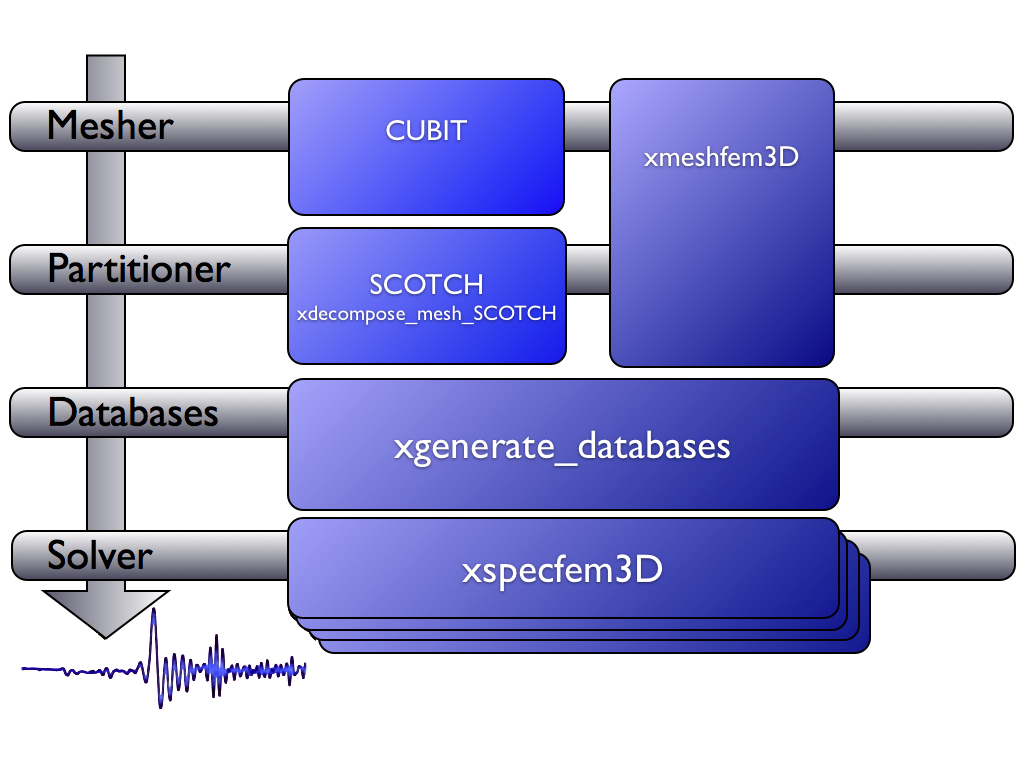
\includegraphics[width=0.8\textwidth]{./images/processing.jpg}
\end{center}
\caption{Workflow for running spectral-element simulations with \href{http://www.geodynamics.org/cig/software/specfem3d}{SPECFEM3D} Version~2.0 `Sesame'.
}
\label{figure:processing}
\end{figure}

\begin{figure}
\begin{center}
\begin{minipage}[t]{0.45\textwidth}
\begin{center}
(a)\\
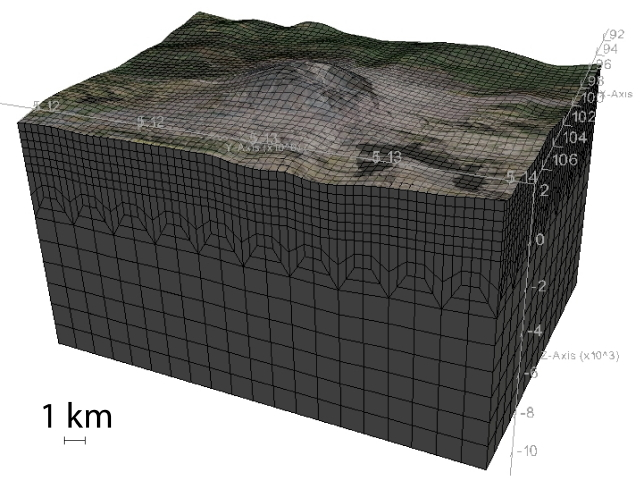
\includegraphics[width=1.\textwidth]{./images/mesh_mountsthelens.jpg}
\end{center}
\end{minipage}
\begin{minipage}[t]{0.45\textwidth}
\begin{center}
(b)\\
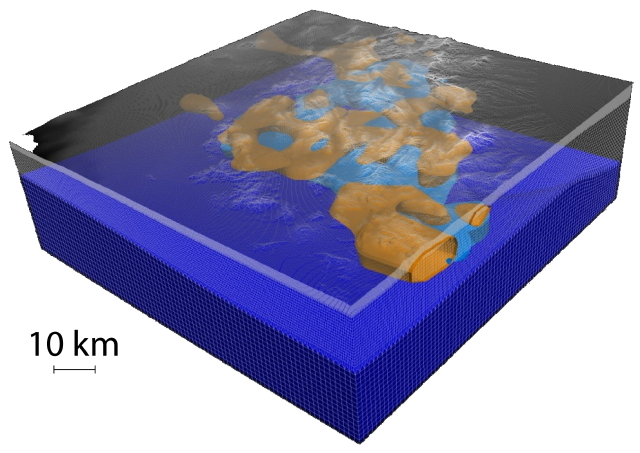
\includegraphics[width=1.\textwidth]{./images/mesh_aquila.jpg}
\end{center}
\end{minipage}
\begin{minipage}[t]{0.45\textwidth}
\begin{center}
(c)\\
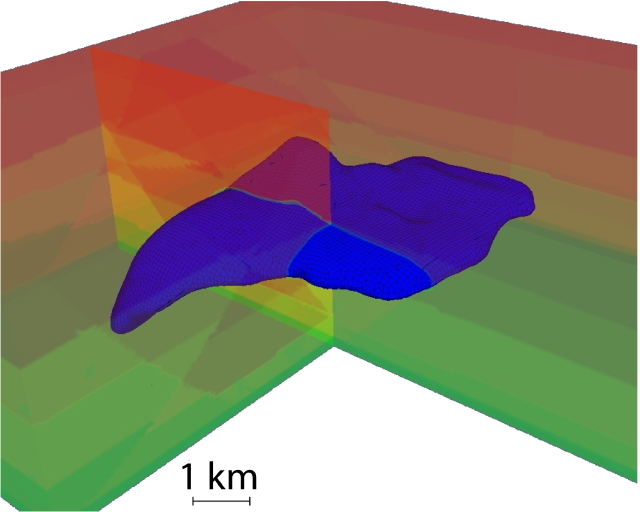
\includegraphics[width=1.\textwidth]{./images/mesh_salt.jpg}
\end{center}
\end{minipage}
\begin{minipage}[t]{0.45\textwidth}
\begin{center}
(d)\\
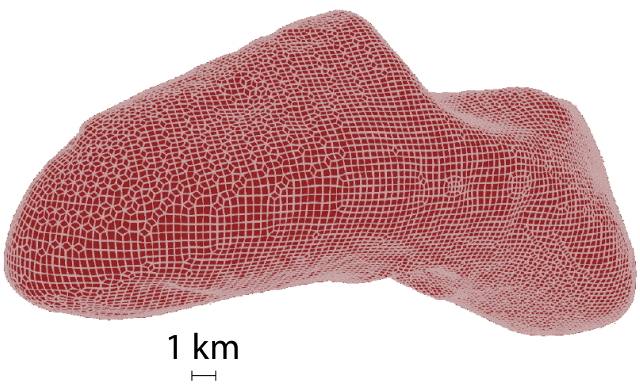
\includegraphics[width=1.\textwidth]{./images/mesh_asteroid.jpg}
\end{center}
\end{minipage}
\begin{minipage}[t]{0.45\textwidth}
\begin{center}
(e)\\
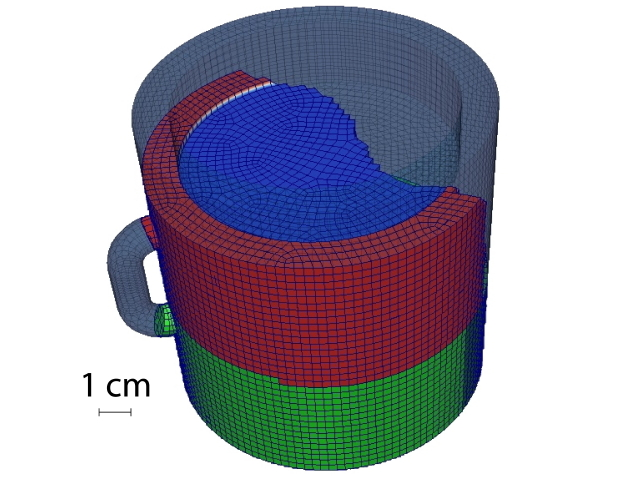
\includegraphics[width=1.\textwidth]{./images/mesh_coffeecup.jpg}
\end{center}
\end{minipage}
\end{center}
\caption{Mesh examples: (a) Mount St.~Helens meshed by hexahedral elements.
The mesh honors surface topography and includes a mesh tripling layer in the middle of the model.
The smallest element size is approximately 280~m.
(b) L'Aquila, Italy, region discretized for high-frequency simulations.
The mesh honors surface and Moho topography and includes two mesh tripling layers.
The yellow and blue volumes denote slower and faster than average wavespeeds, respectively.
(c) Salt dome body meshed inside an exploration model for a SEG/EAGE benchmark test.
(d) 3D hexahedral mesh of the asteroid 433-Eros.
(e) Arbitrarily-shaped mesh for coupled solid-fluid simulations involving a coffee cup.
}
\label{figure:mountsthelens}
\end{figure}

\begin{figure}
\begin{center}
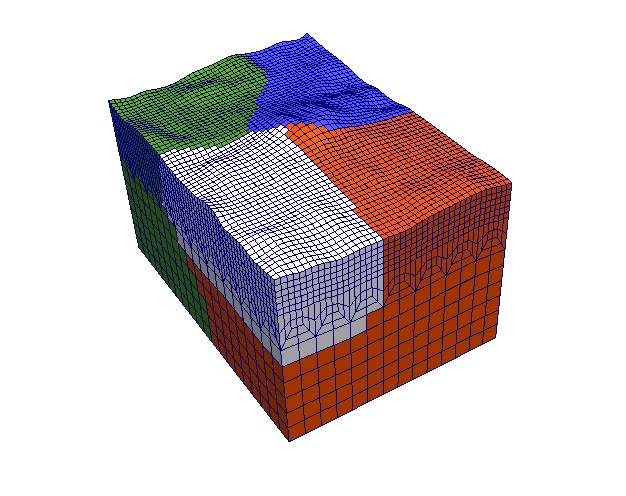
\includegraphics[width=0.49\textwidth]{./images/mount-partitions.jpg}
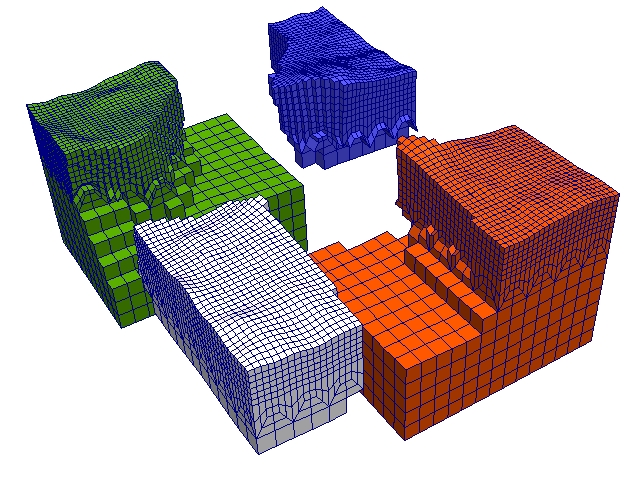
\includegraphics[width=0.49\textwidth]{./images/mount-partitions2.jpg}
\end{center}
\caption{Mount St.~Helens mesh partitioned and load balanced to run in parallel on four cores.
The four partitions are indicated by different colors.
}
\label{figure:partitions}
\end{figure}

\begin{figure}
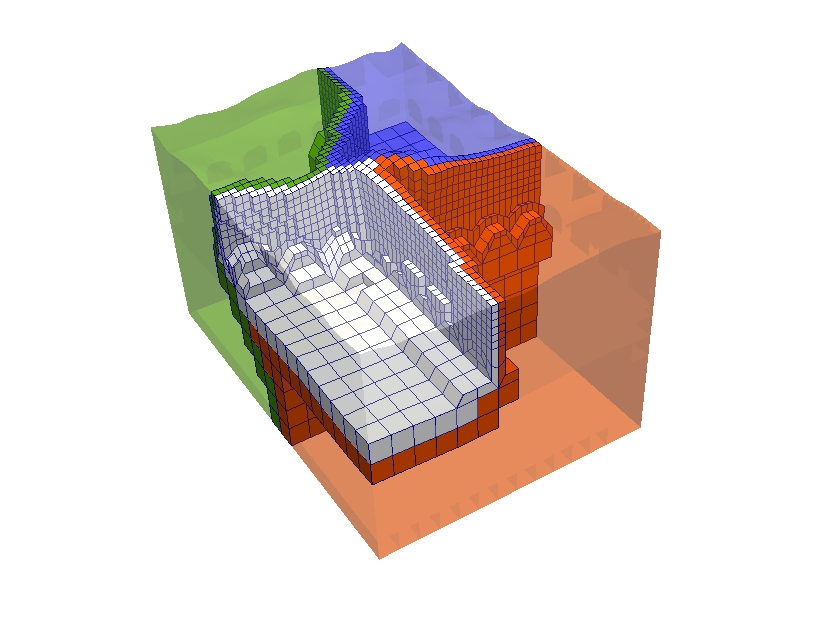
\includegraphics[width=0.49\textwidth]{./images/mesh_inner_outer.jpg}
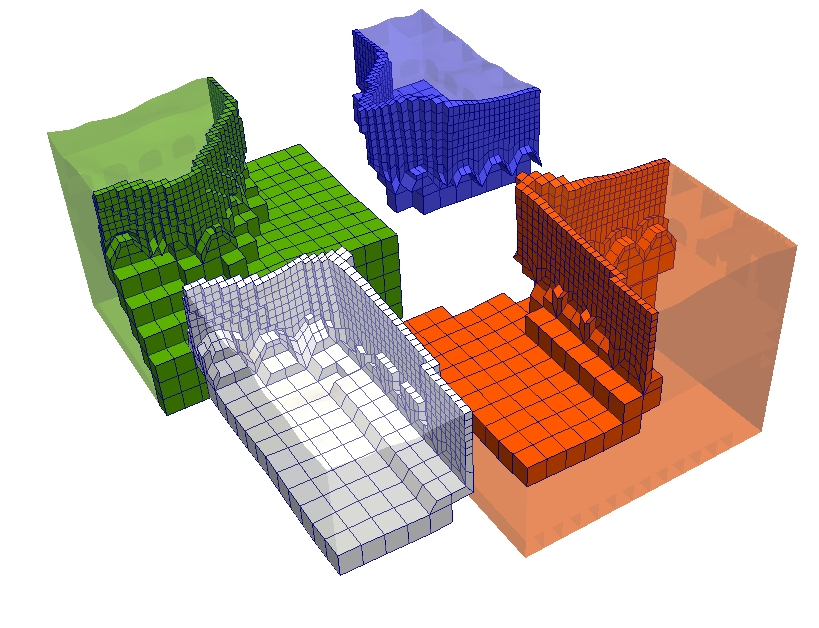
\includegraphics[width=0.49\textwidth]{./images/mesh_inner_outer2.jpg}
\caption{
Outer (highlighted) and inner (transparent colors) elements for the mesh shown in
Figure~\ref{figure:partitions}. Outer elements have at least one point in common with an element
from another slice and must therefore be computed first, before initiating non-blocking MPI
communications.
While MPI messages are traveling across the computer network,
simultaneous computations are performed on inner elements.
Non-blocking MPI communication is crucial to obtain good scaling
results for simulations running on a large number of parallel cores.}
\label{inner_outer_elements}
\end{figure}

\begin{figure}
\begin{center}
\begin{minipage}[t]{0.45\textwidth}
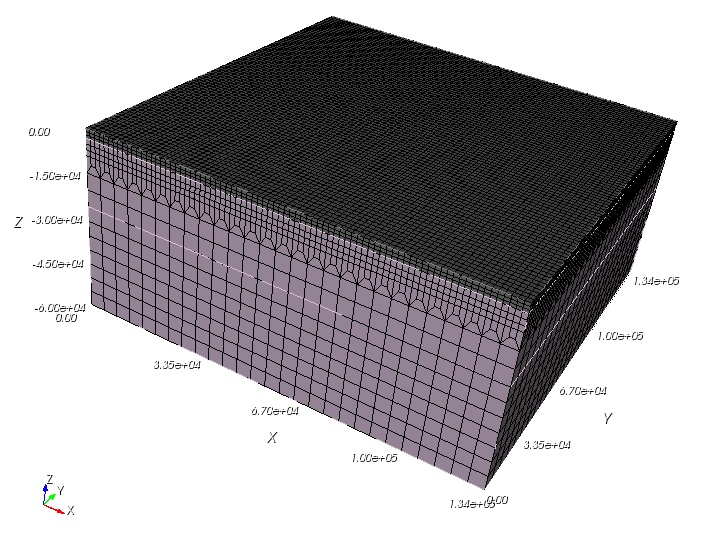
\includegraphics[width=1.\textwidth]{./images/2lay_mesh_boundary_fig8.jpg} \\
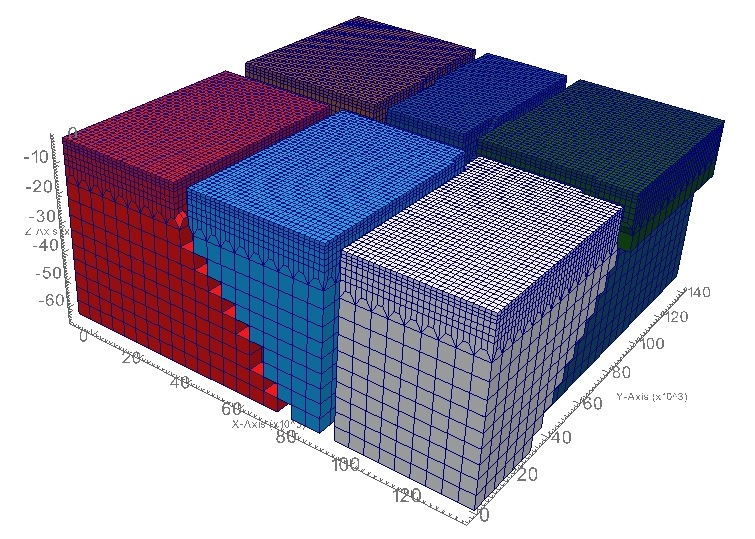
\includegraphics[width=1.\textwidth]{./images/2lay_mesh_partitions.jpg}
\end{minipage}
\begin{minipage}[t]{0.45\textwidth}
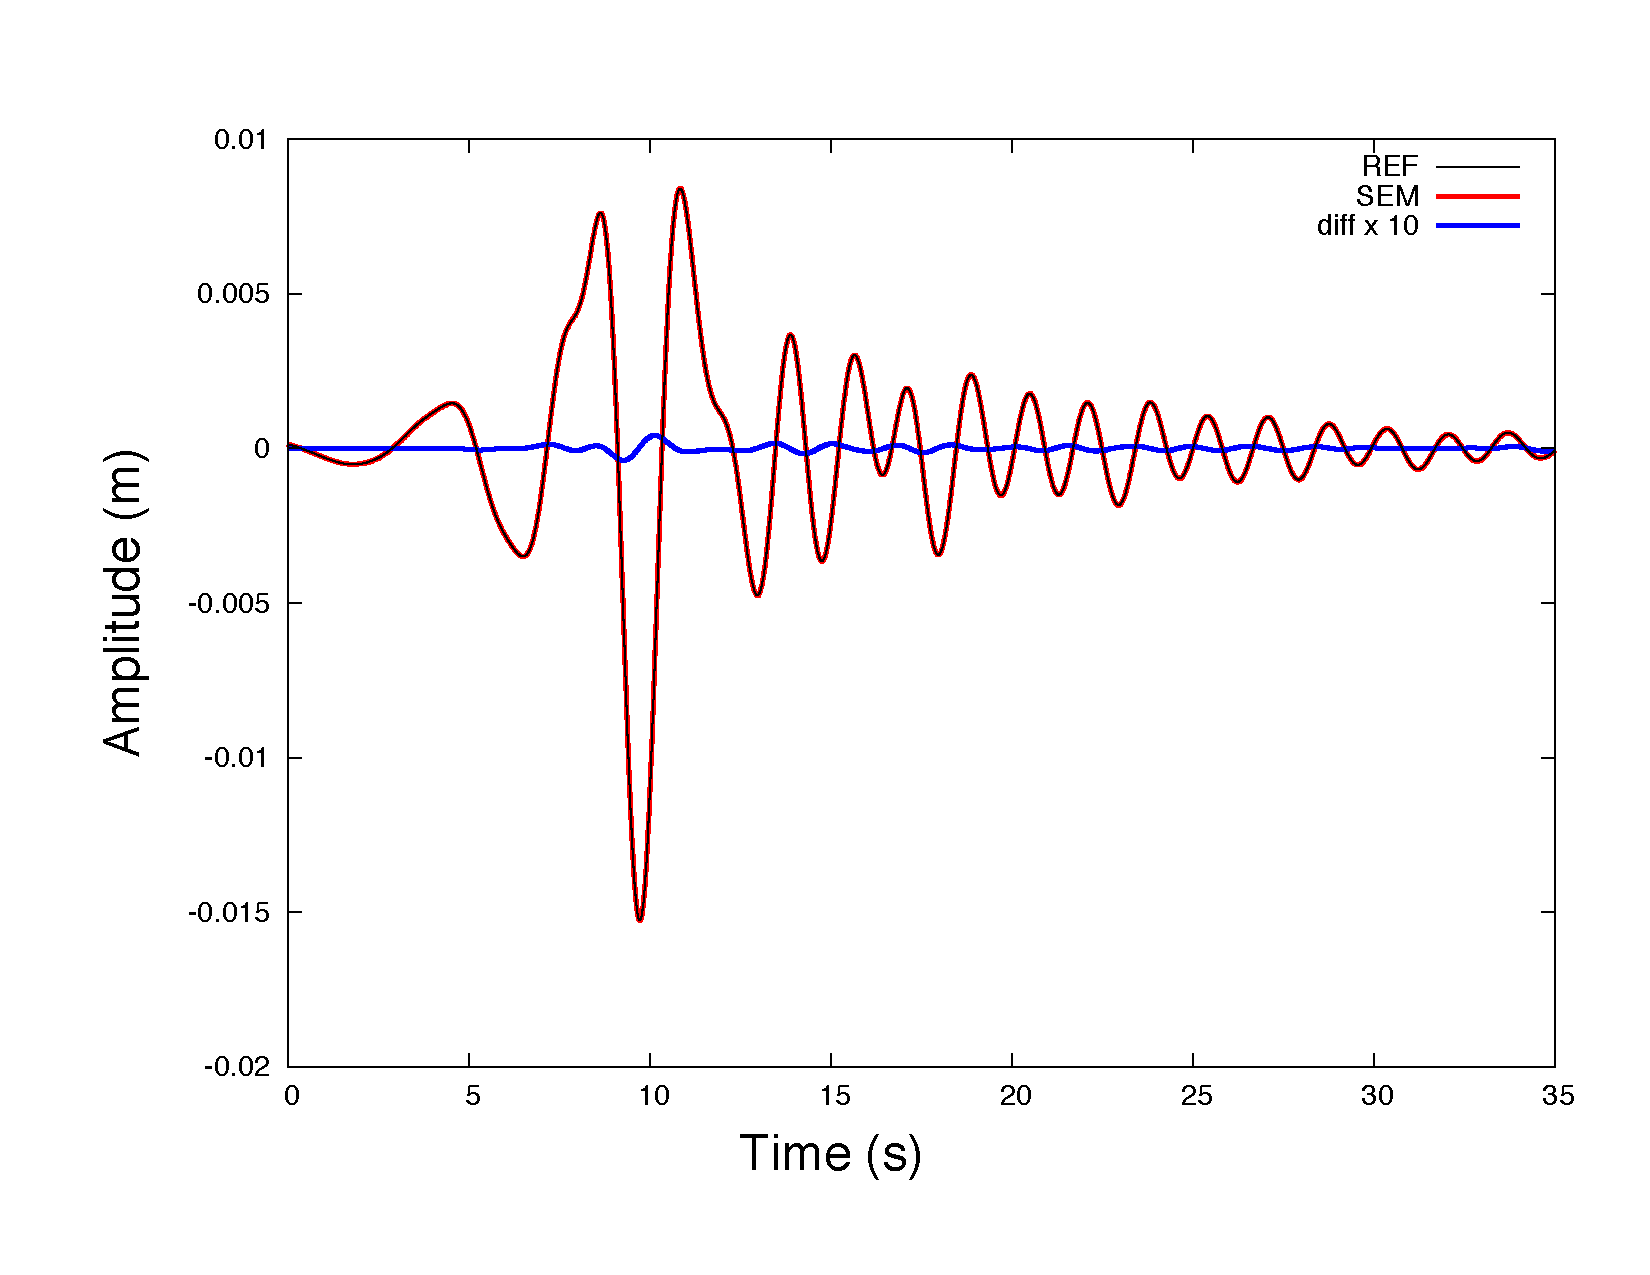
\includegraphics[width=1.\textwidth]{./images/2lay_traces55_R.pdf} \\
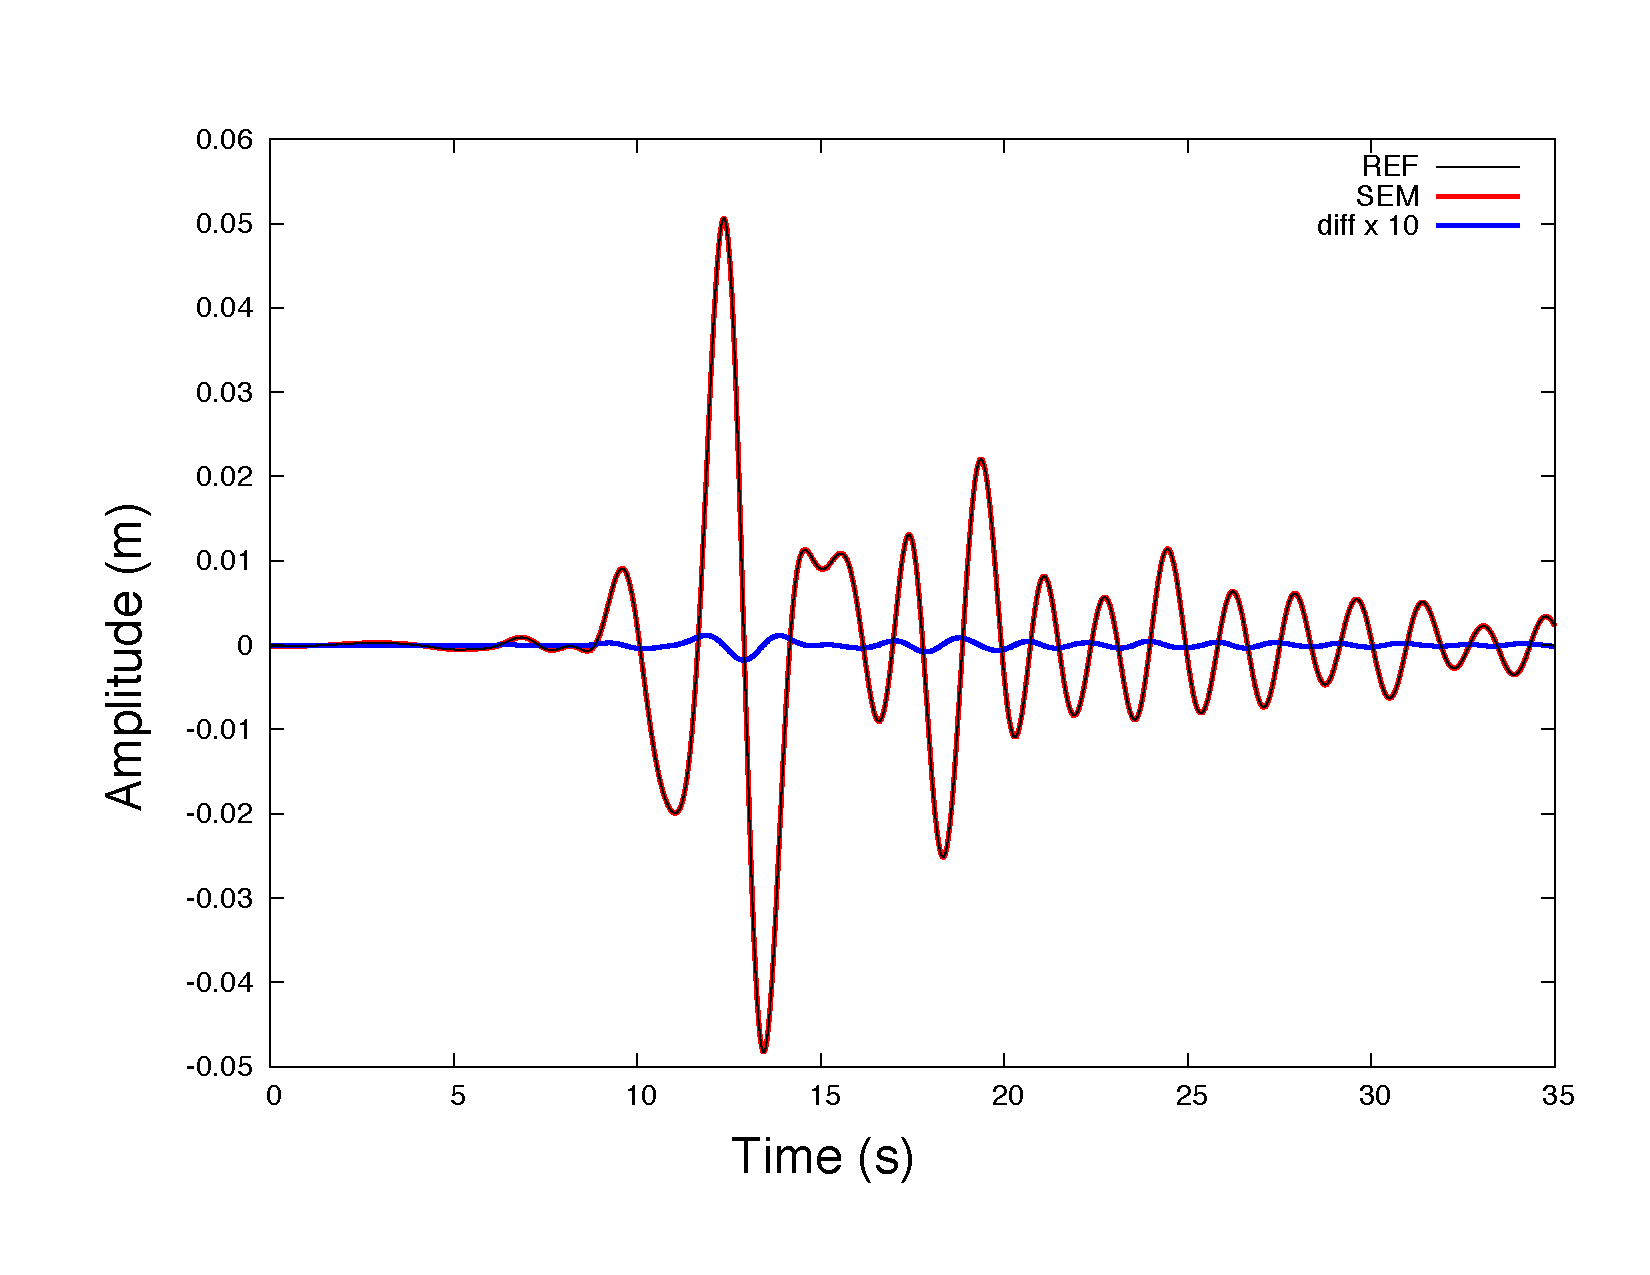
\includegraphics[width=1.\textwidth]{./images/2lay_traces31_R.pdf}
\end{minipage}
\end{center}
\caption{Validation for a two-layer mesh (left, top), using six partitions (left, bottom),
and seismograms recorded at the surface at horizontal distances of 2.39~km (right, top) and 31.11~km (right, bottom).
Plotted are radial displacements (SEM, red) against reference solutions (REF, black) from \cite{KoTr99},
as well as their exaggerated differences (blue) .
}
\label{figure:validation}
\end{figure}


\begin{figure}
\begin{center}
\begin{minipage}[t]{0.49\textwidth}
\begin{center}
(a) \\
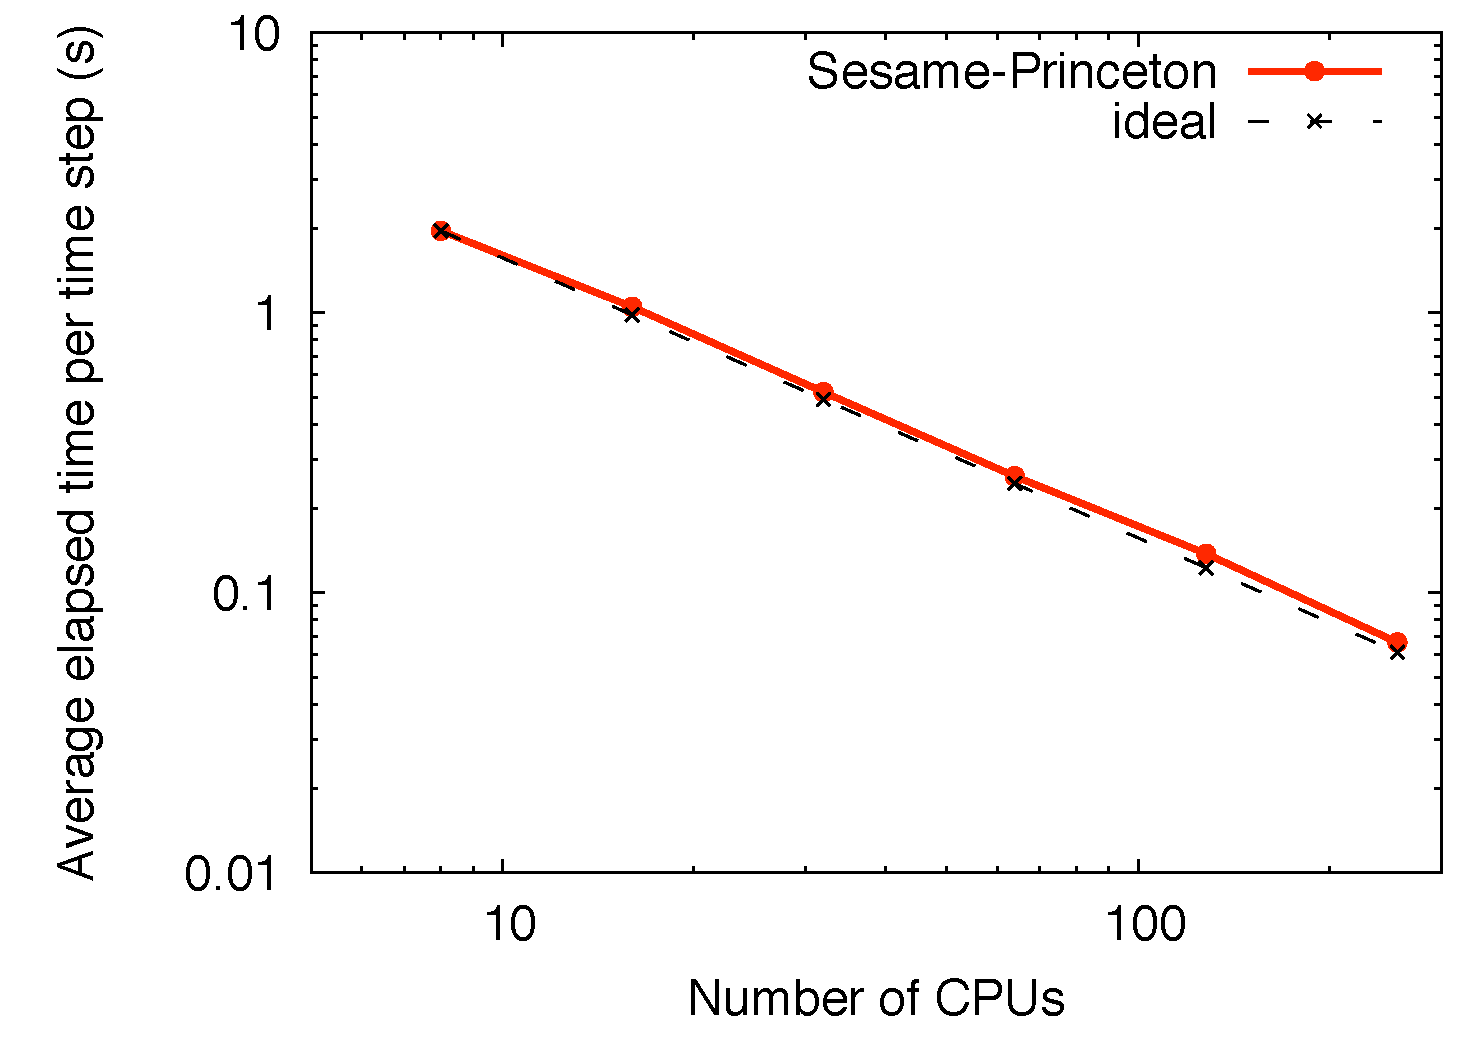
\includegraphics[width=.9\textwidth]{./images/output_elapsed_time_strong.pdf}
\end{center}
\end{minipage}
\begin{minipage}[t]{0.49\textwidth}
\begin{center}
(b) \\
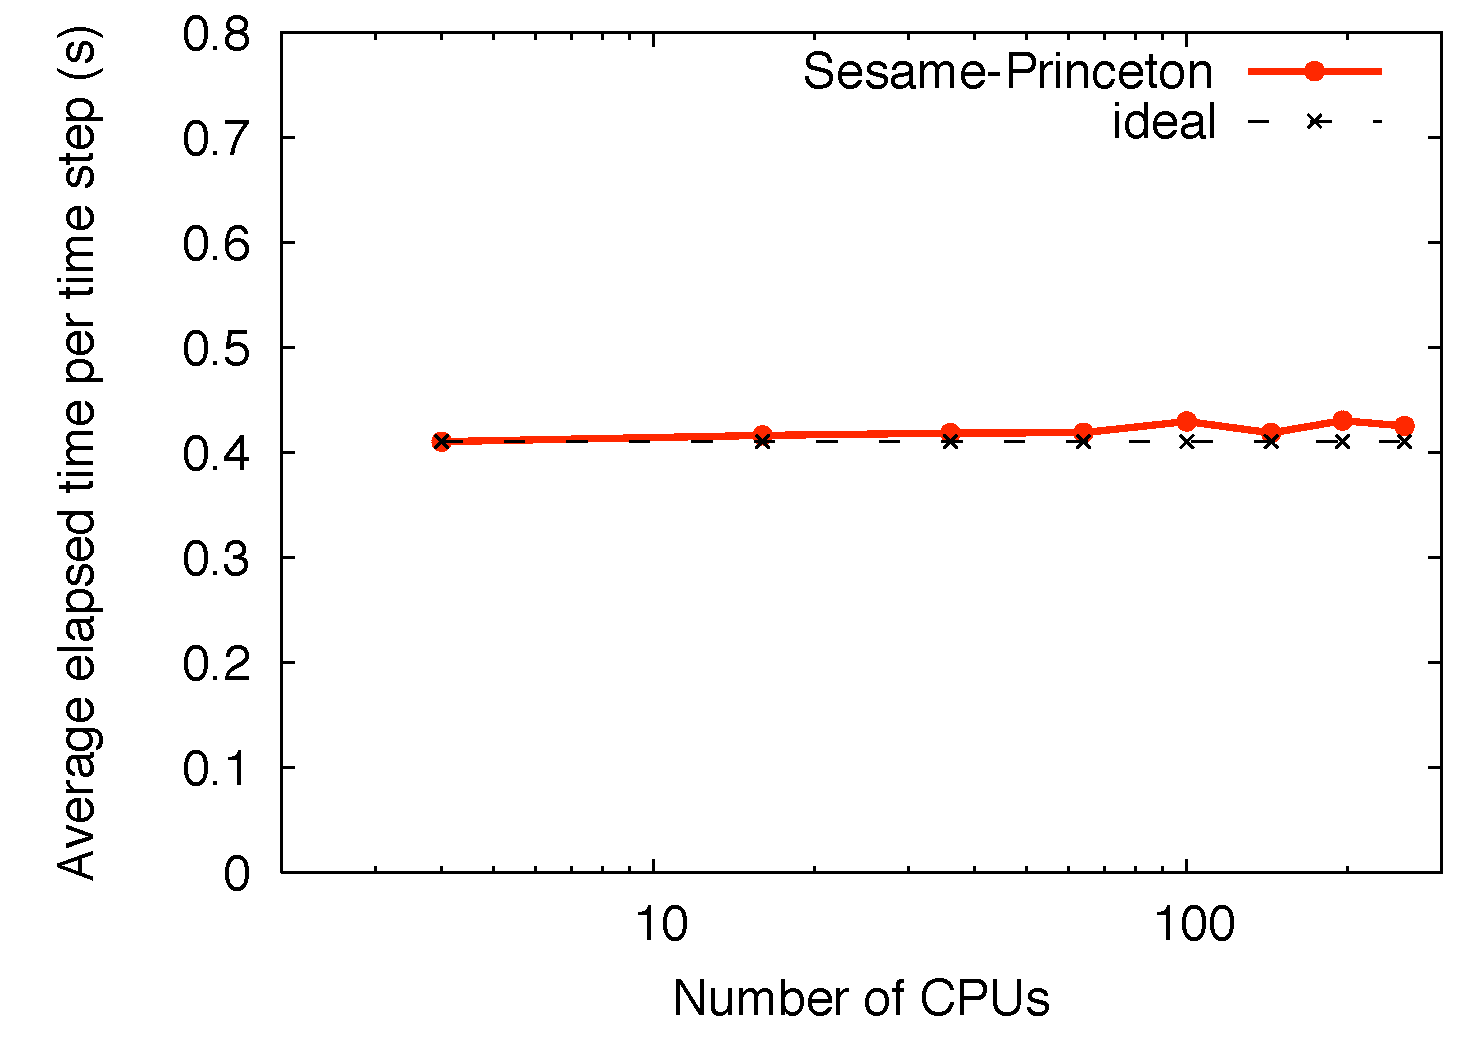
\includegraphics[width=.9\textwidth]{./images/output_elapsed_time_weak.pdf}
\end{center}
\end{minipage}
\end{center}
\caption{CPU scaling results for the model shown in Fig.~\ref{figure:validation}, (a) using a fixed total problem size (strong scaling) and (b) a fixed problem size per processor (weak scaling) for up to 256 cores.
Perfect weak scaling deviates slightly from a straight line,
because a larger number of processors involves more MPI buffers and therefore more computational overhead.
}
\label{figure:scaling}
\end{figure}


\begin{figure}
\begin{center}
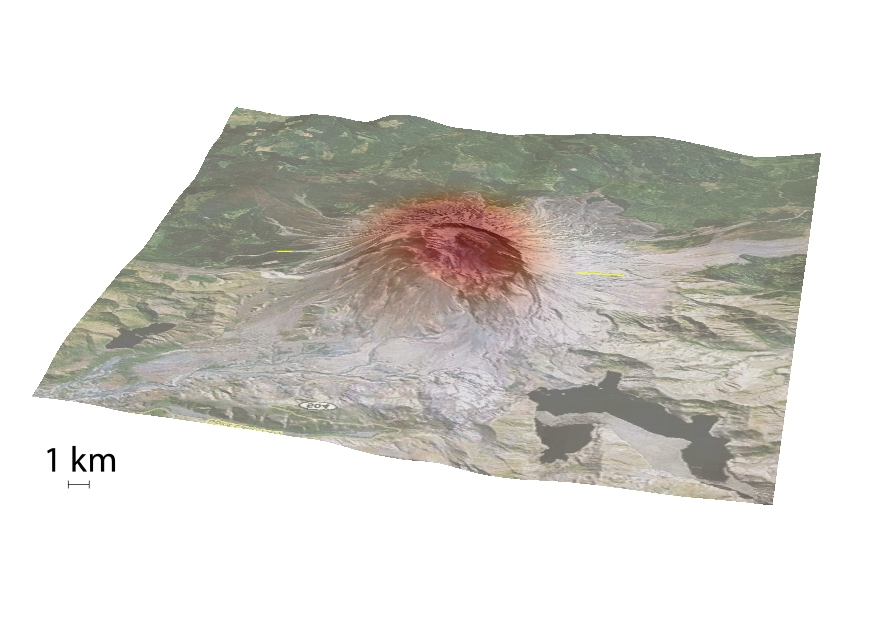
\includegraphics[width=0.45\textwidth]{./images/mount2.jpg}
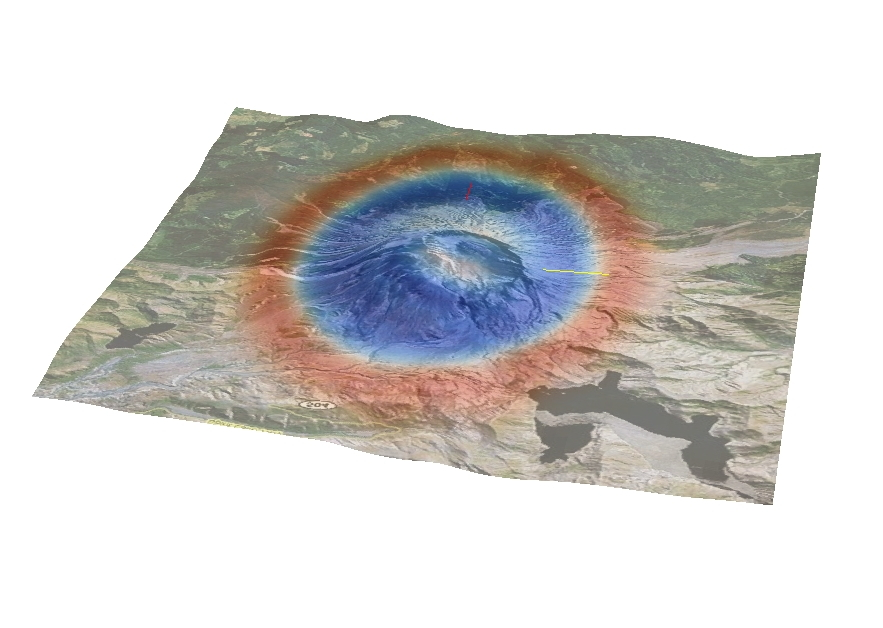
\includegraphics[width=0.45\textwidth]{./images/mount3.jpg}
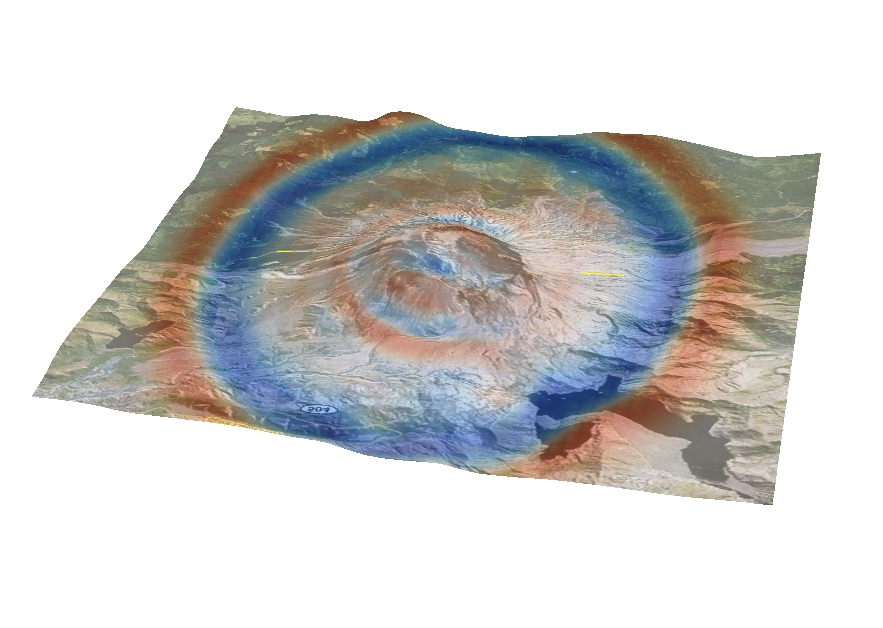
\includegraphics[width=0.45\textwidth]{./images/mount4.jpg}
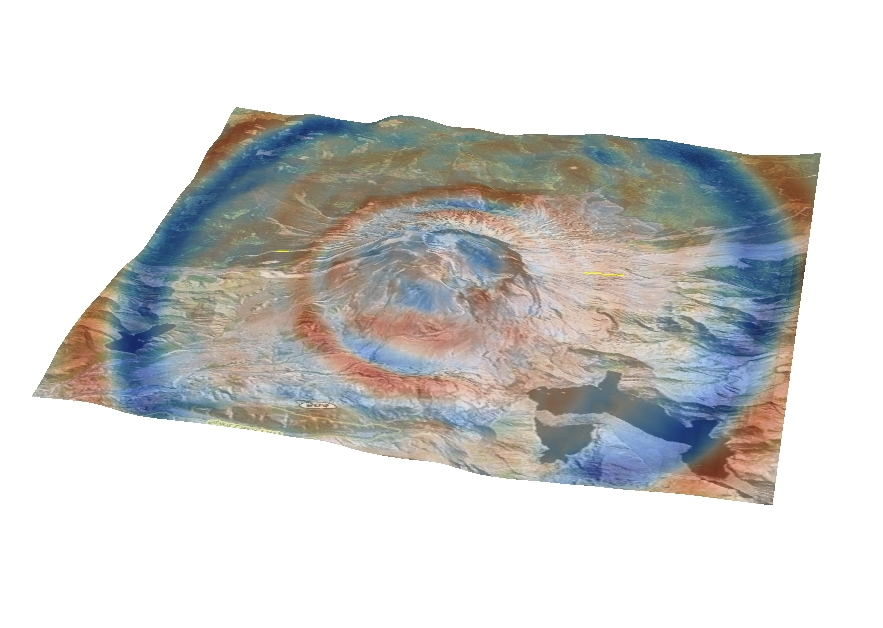
\includegraphics[width=0.45\textwidth]{./images/mount5.jpg}
\end{center}
\caption{Wavefield snapshots around Mount St.~Helens. Plotted are vertical displacements (up/down colored red/blue respectively) at the free surface of the model.
}
\label{figure:mountsnapshots}
\end{figure}


\begin{figure}
\begin{center}
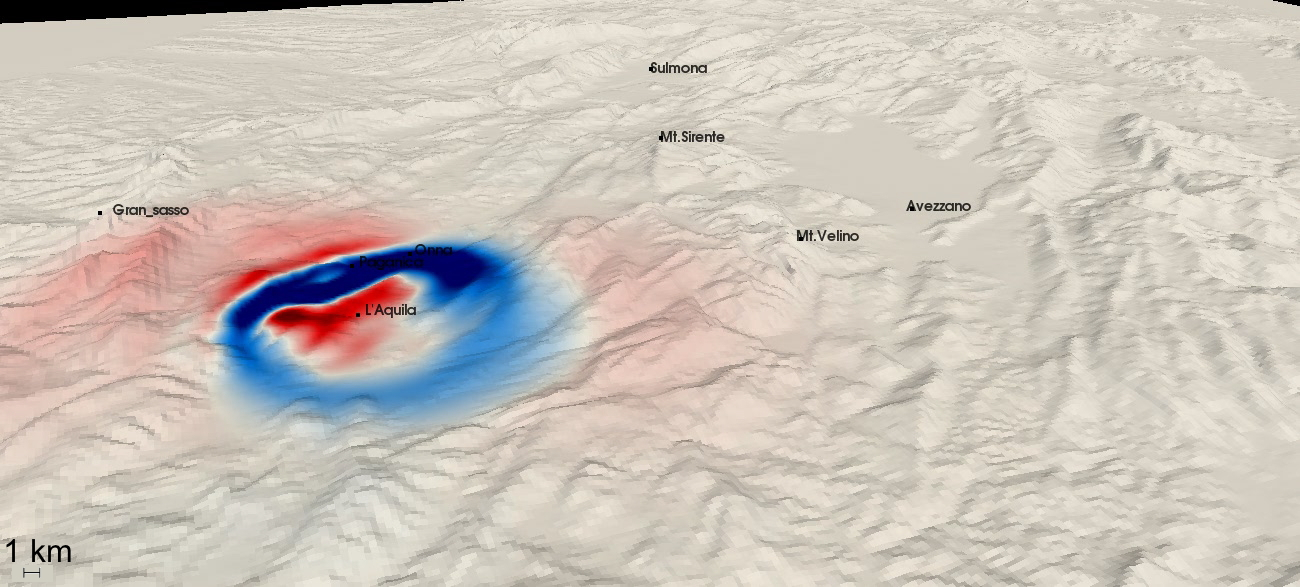
\includegraphics[width=0.45\textwidth]{./images/aquila_1d_7000source-1.jpg}
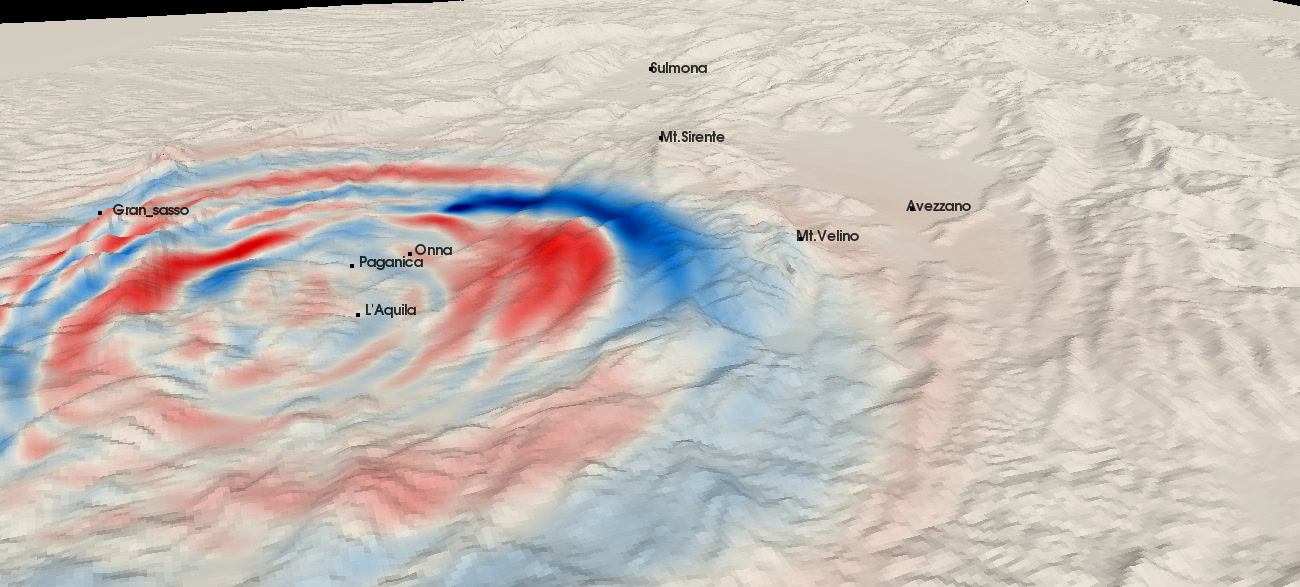
\includegraphics[width=0.45\textwidth]{./images/aquila_1d_7000source-2.jpg}
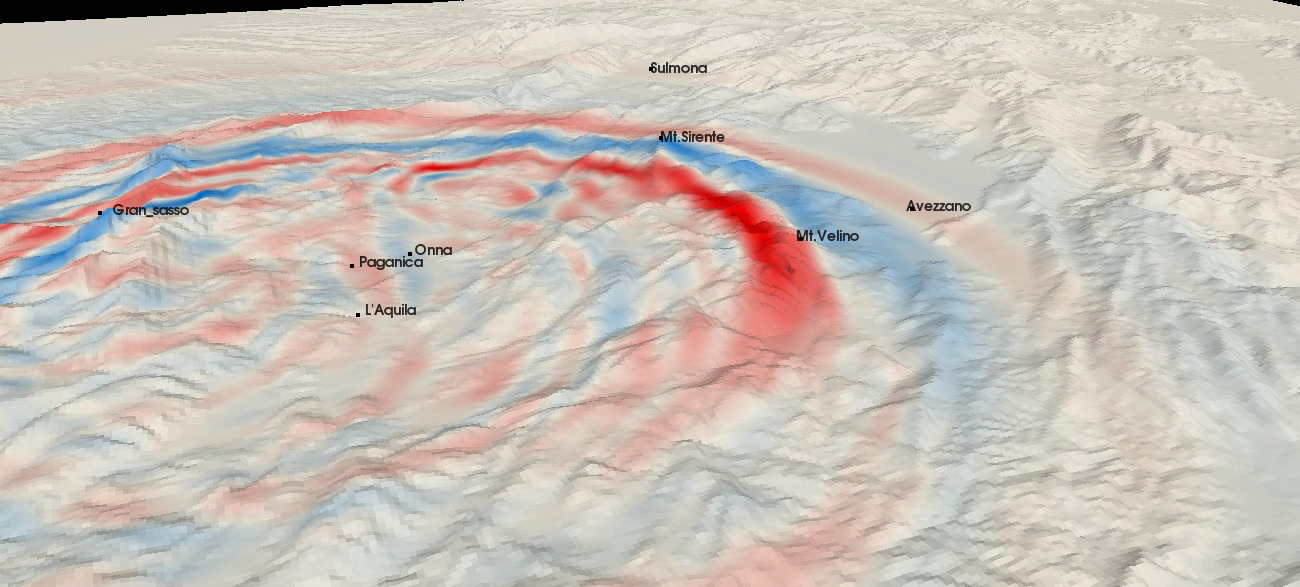
\includegraphics[width=0.45\textwidth]{./images/aquila_1d_7000source-3.jpg}
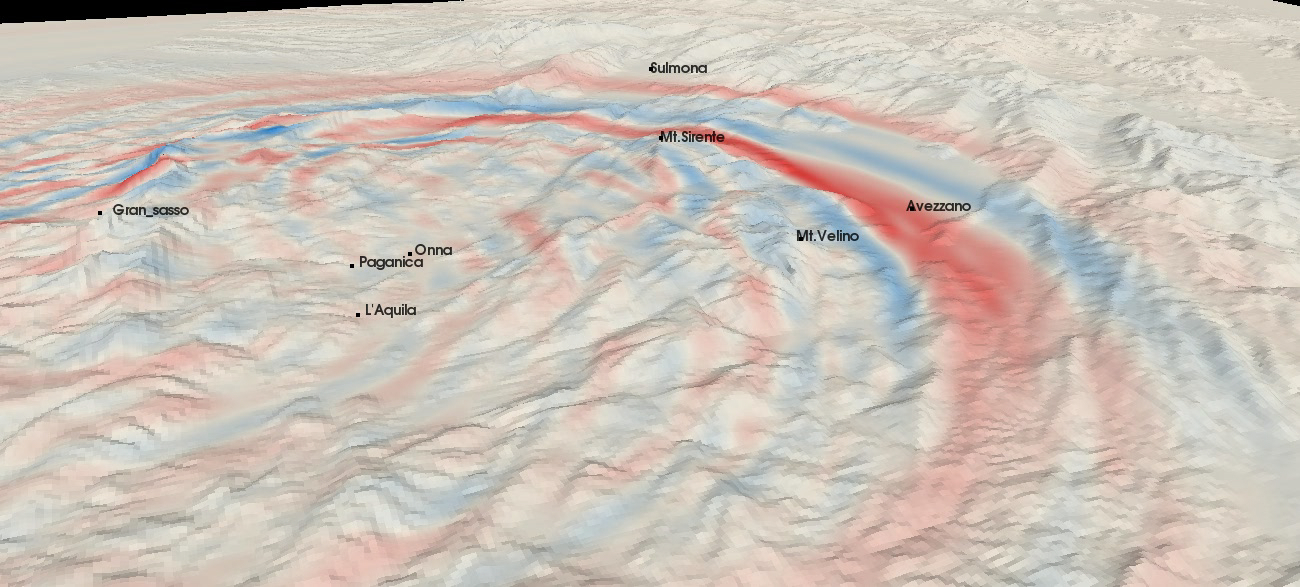
\includegraphics[width=0.45\textwidth]{./images/aquila_1d_7000source-4.jpg}
\end{center}
\caption{Wavefield snapshots for the April~6, 2009, L'Aquila earthquake,
taken after 6~s, 11~s, 16~s and 21~s.
Plotted are vertical displacements (up/down as red/blue).
}
\label{figure:aquila}
\end{figure}

\begin{figure}
\begin{center}
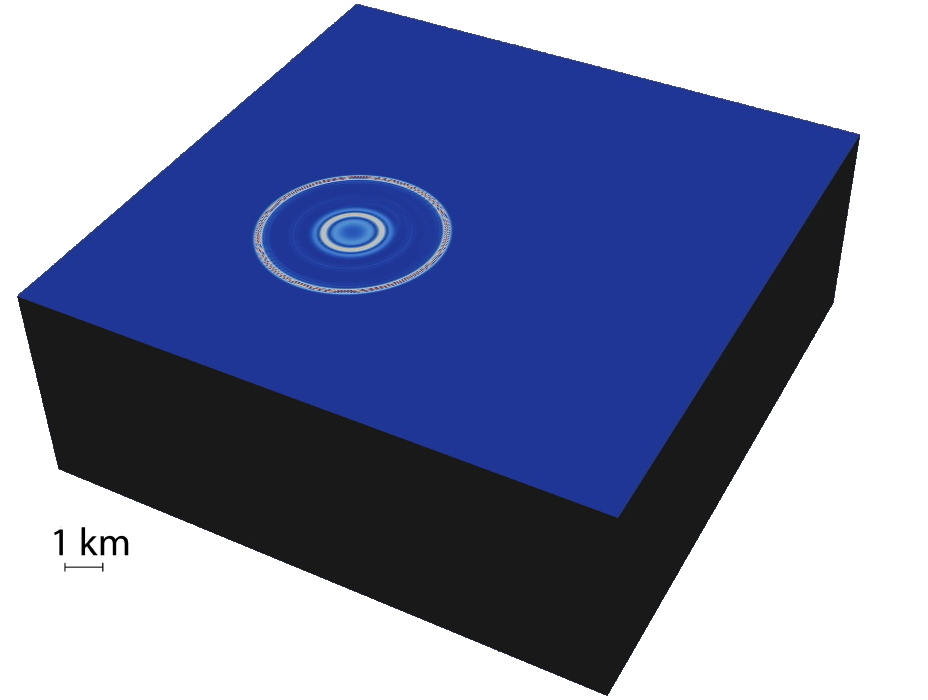
\includegraphics[width=0.45\textwidth]{./images/salt-mesh_1_0005.jpg}
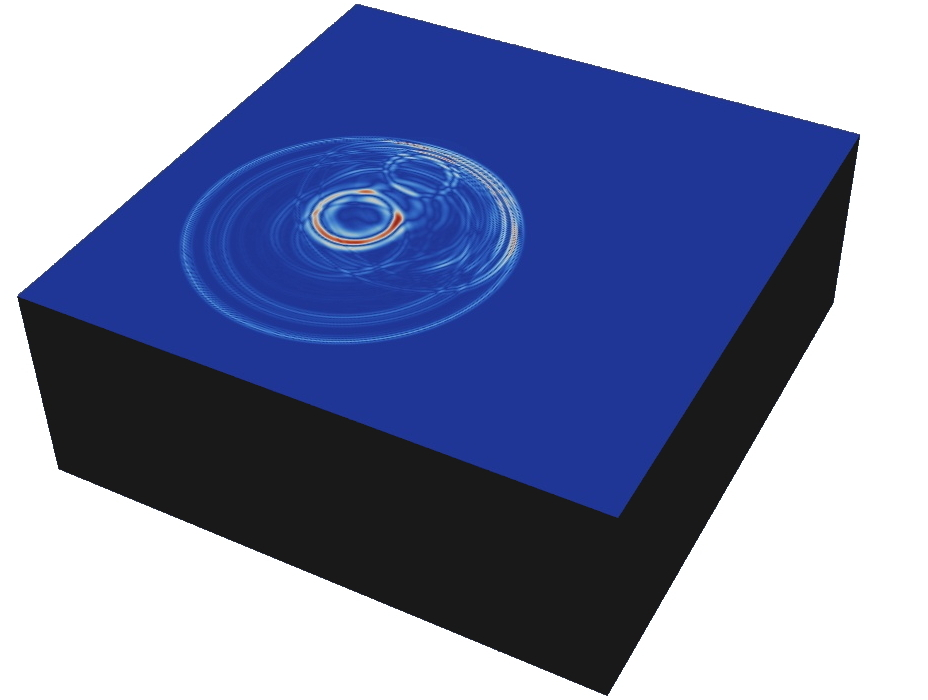
\includegraphics[width=0.45\textwidth]{./images/salt-mesh_1_0010.jpg}
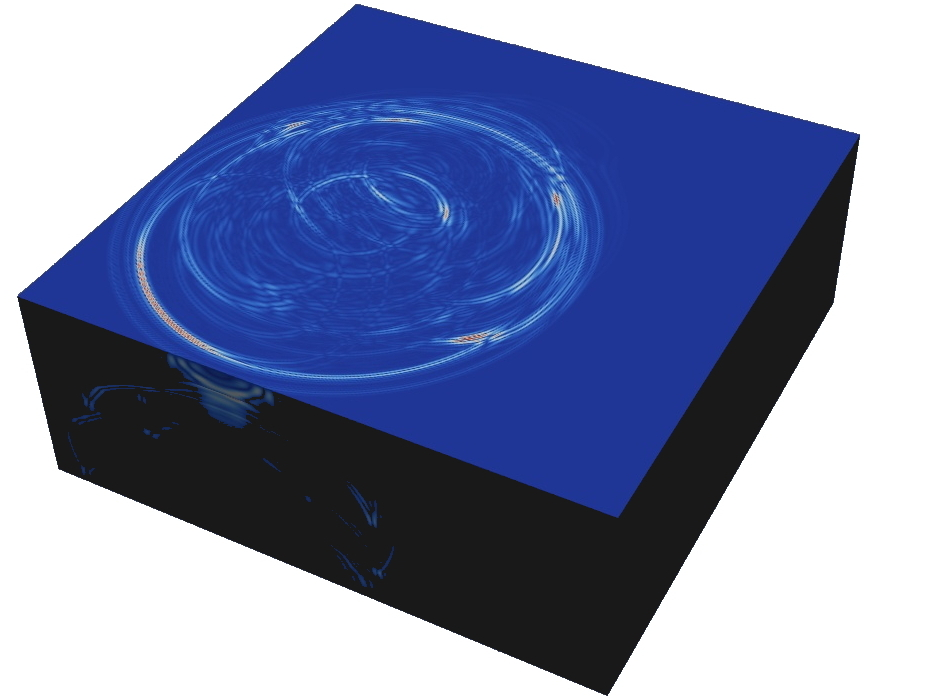
\includegraphics[width=0.45\textwidth]{./images/salt-mesh_1_0015.jpg}
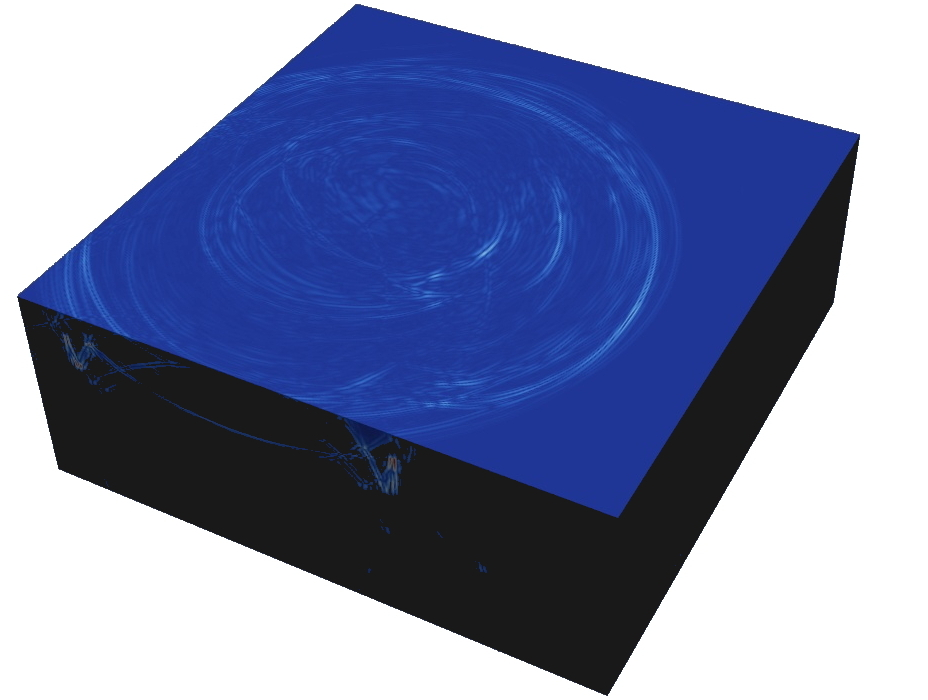
\includegraphics[width=0.45\textwidth]{./images/salt-mesh_1_0020.jpg}
\end{center}
\caption{Wavefield snapshots for an exploration geophysics simulation taken after 5~s,
10~s, 15~s and 20~s.
Plotted are vertical velocities at the free surface of the water layer.
}
\label{figure:saltdome}
\end{figure}

\begin{figure}
\begin{center}
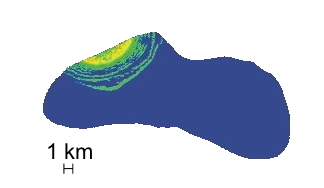
\includegraphics[width=0.45\textwidth]{./images/asteroid_1.jpg}
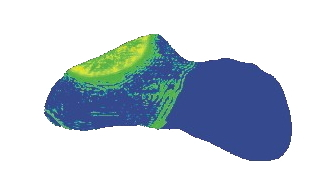
\includegraphics[width=0.45\textwidth]{./images/asteroid_2.jpg}
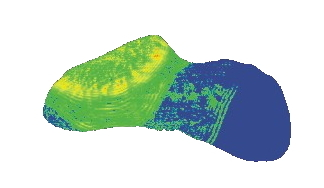
\includegraphics[width=0.45\textwidth]{./images/asteroid_3.jpg}
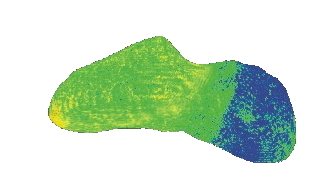
\includegraphics[width=0.45\textwidth]{./images/asteroid_4.jpg}
\end{center}
\caption{Wavefield snapshots for an asteroid simulation taken after 3~s,
4.5~s, 6.5~s and 10.5~s.
Plotted is the norm of the velocity at the free surface of the asteroid.
}
\label{figure:asteroid}
\end{figure}

\begin{figure}
\begin{center}
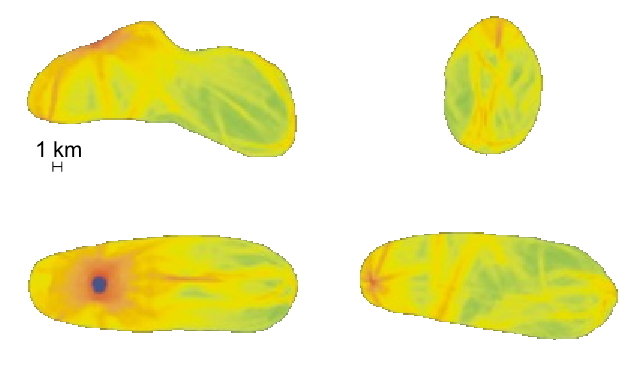
\includegraphics[width=1.\textwidth]{./images/asteroid_shakemap1.jpg}
\end{center}
\caption{ShakeMap views for an asteroid simulation.
Plotted are different views of the peak ground accelerations at the free surface of the asteroid.
}
\label{figure:asteroidshakemap}
\end{figure}


\begin{figure}
\begin{center}
\begin{minipage}[t]{0.49\textwidth}
\begin{center}
(a)\\
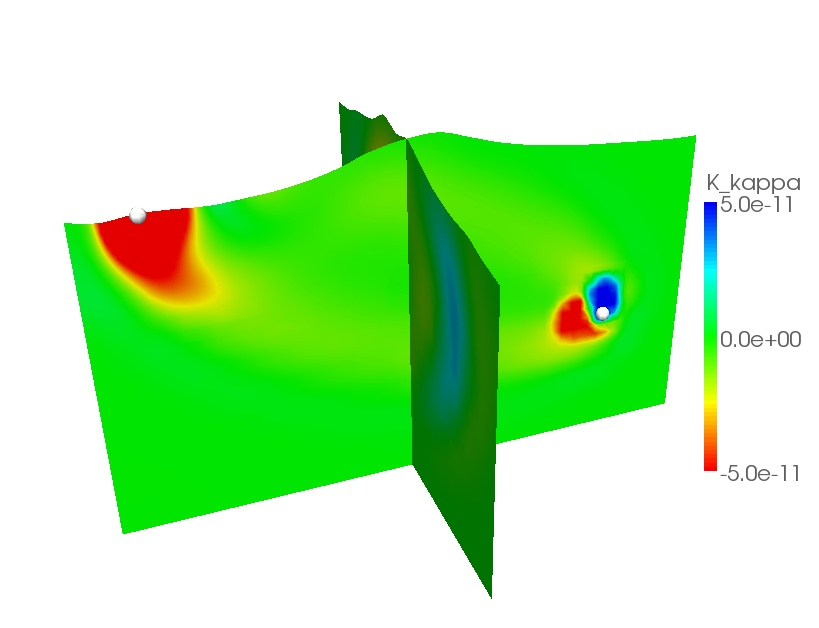
\includegraphics[width=1.\textwidth]{./images/mount_kappa_kernel.jpg} \\
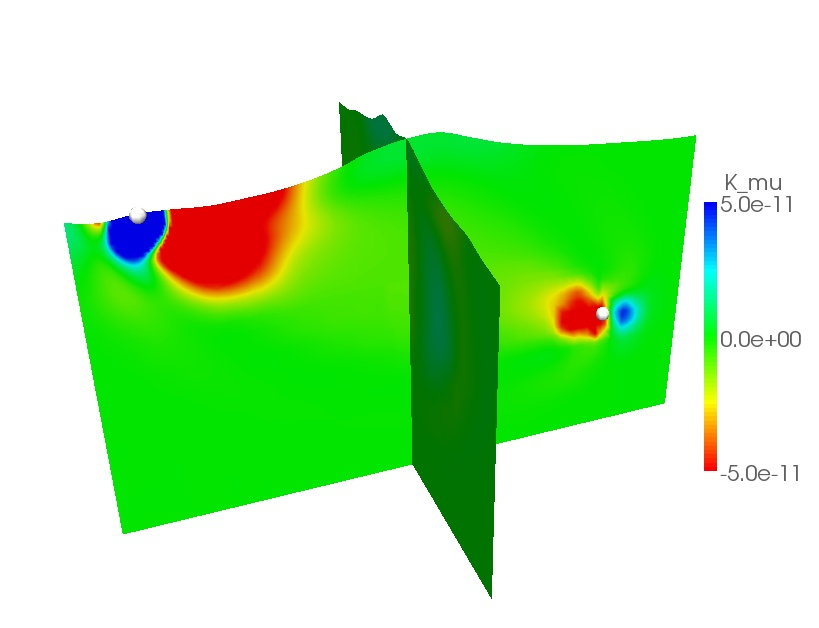
\includegraphics[width=1.\textwidth]{./images/mount_mu_kernel.jpg}\\
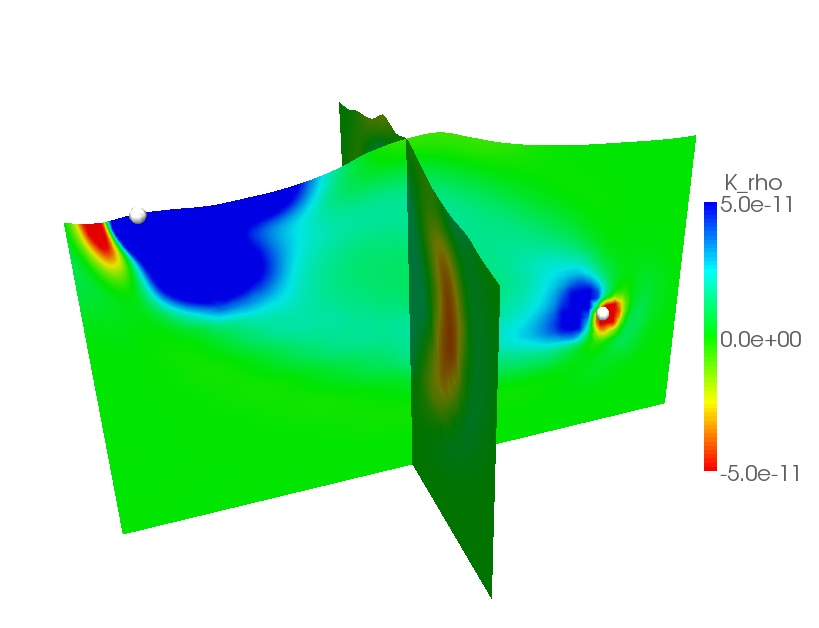
\includegraphics[width=1.\textwidth]{./images/mount_rho_kernel.jpg}
\end{center}
\end{minipage}
\begin{minipage}[t]{0.49\textwidth}
\begin{center}
(b)\\
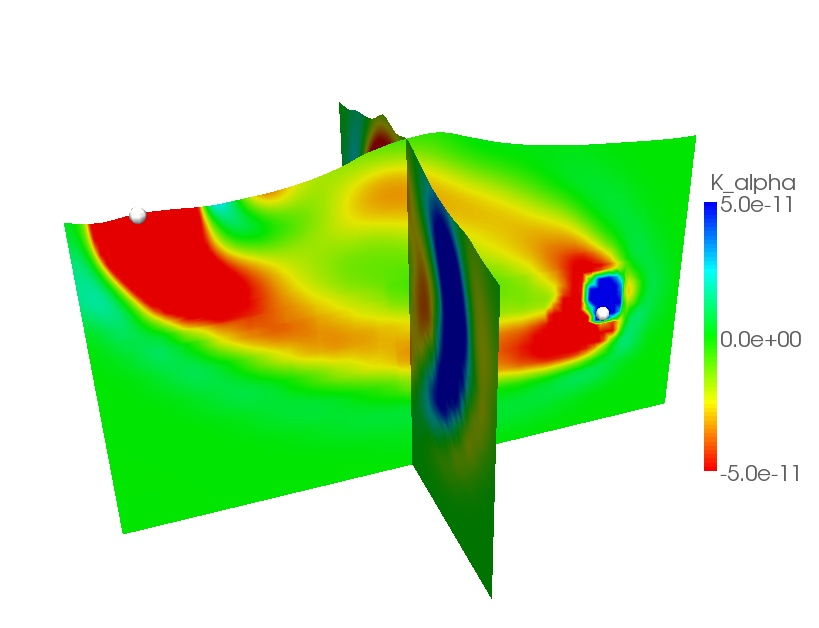
\includegraphics[width=1.\textwidth]{./images/mount_alpha_kernel.jpg} \\
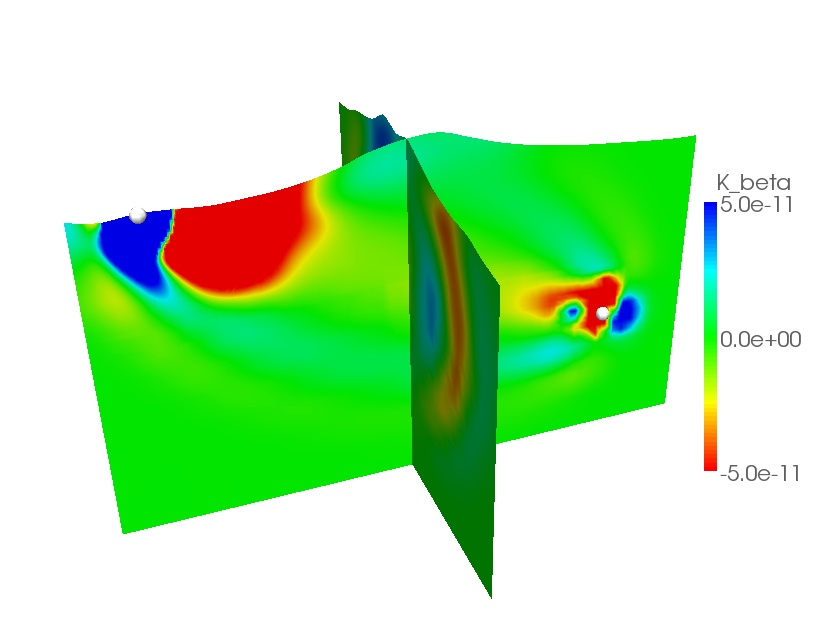
\includegraphics[width=1.\textwidth]{./images/mount_beta_kernel.jpg} \\
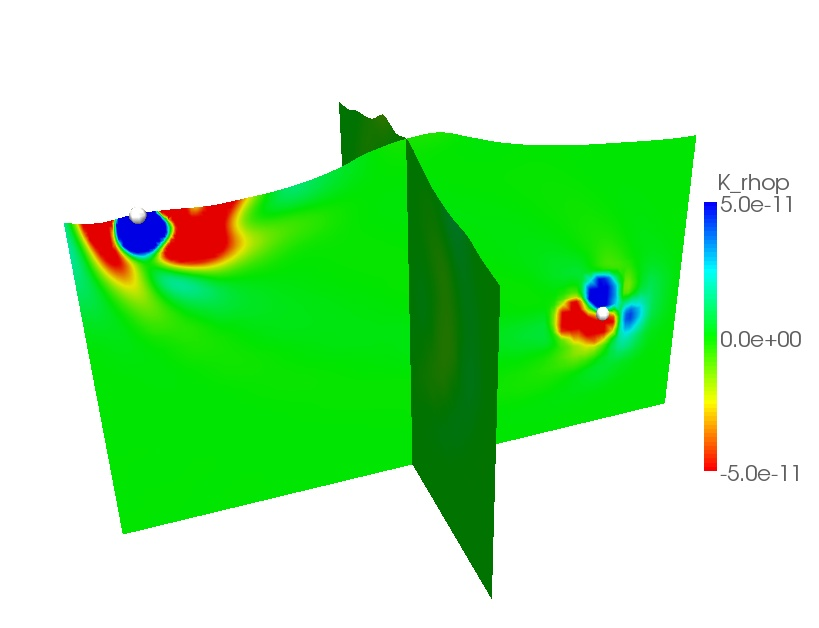
\includegraphics[width=1.\textwidth]{./images/mount_rhop_kernel.jpg}
\end{center}
\end{minipage}
\end{center}
\caption{Traveltime sensitivity to elastic structure.
Fr\'echet derivatives for isotropic parameterizations (a) $K_\kappa$, $K_\mu$ \& $K_\rho$ and (b) $K_\alpha$, $K_\beta$ \& $K'_{\rho}$ are compared in a model of Mount St.~Helens using traveltime adjoint sources for the P wave.
Shown are vertical cross sections through the source-receiver line and perpendicular to this line.
}
\label{figure:kerneliso}
\end{figure}


\begin{figure}
\begin{center}
\begin{minipage}[t]{0.49\textwidth}
\begin{center}
(a)\\
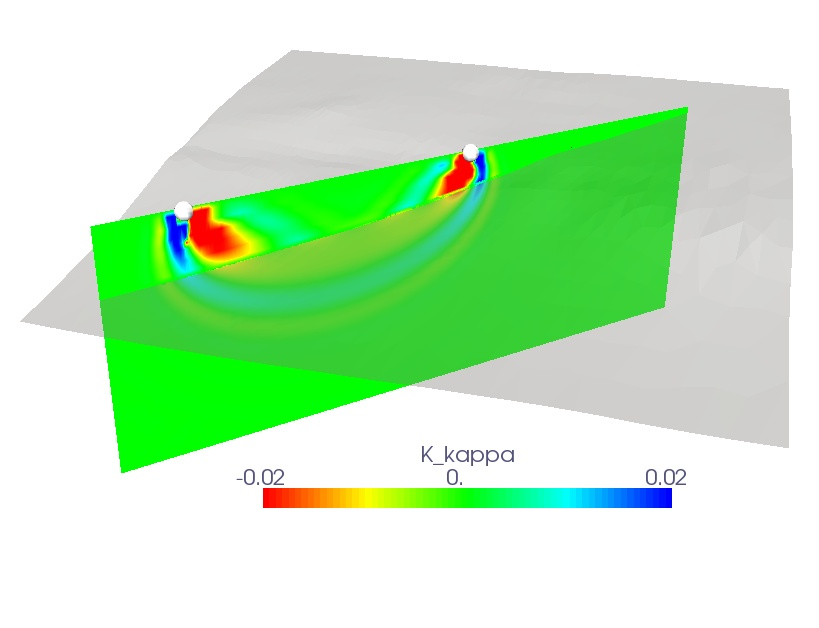
\includegraphics[width=1.\textwidth]{./images/pearl_kappa_kernel.jpg}\\
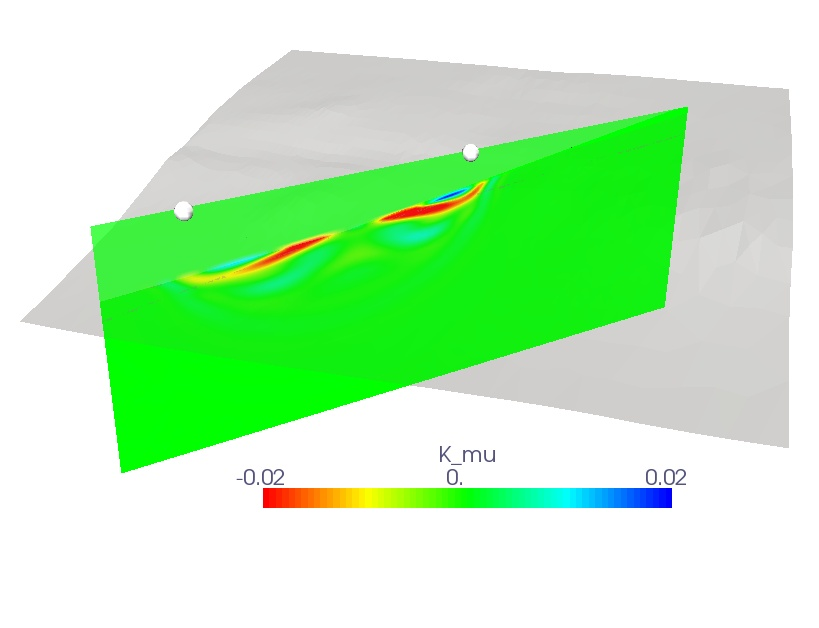
\includegraphics[width=1.\textwidth]{./images/pearl_mu_kernel.jpg}\\
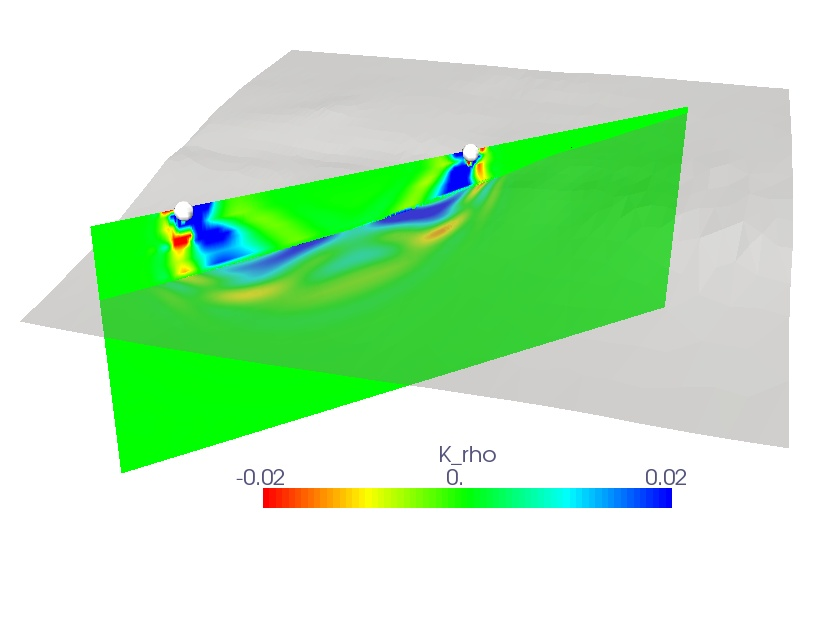
\includegraphics[width=1.\textwidth]{./images/pearl_rho_kernel.jpg}
\end{center}
\end{minipage}
\begin{minipage}[t]{0.49\textwidth}
\begin{center}
(b)\\
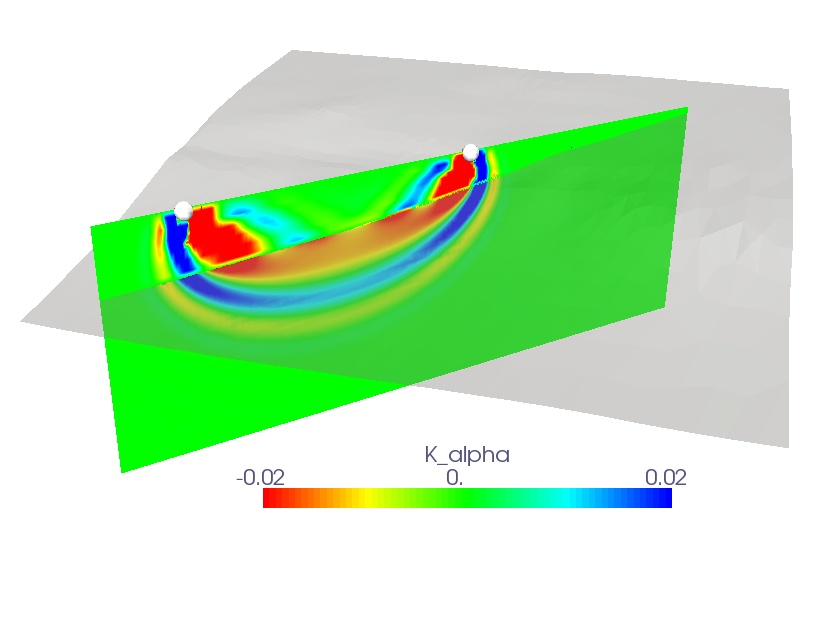
\includegraphics[width=1.\textwidth]{./images/pearl_alpha_kernel.jpg}\\
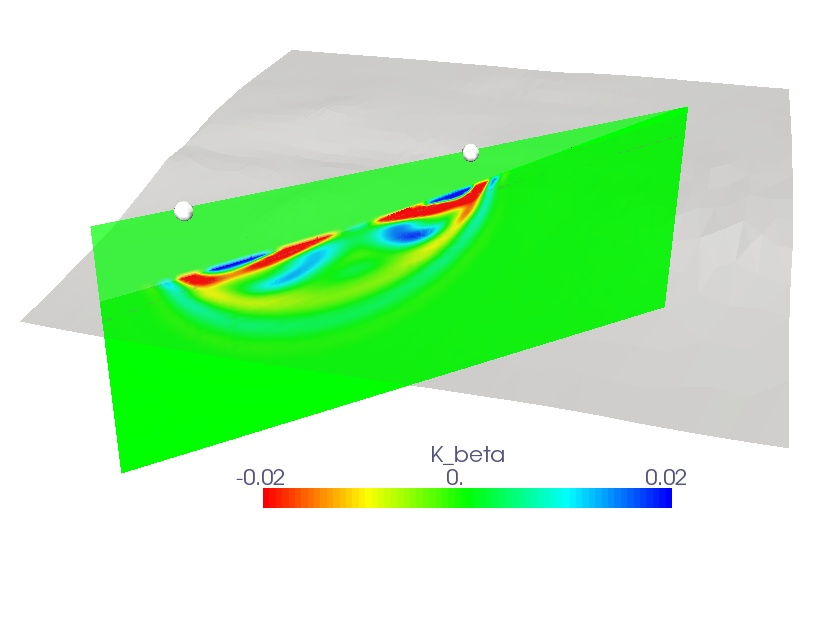
\includegraphics[width=1.\textwidth]{./images/pearl_beta_kernel.jpg}\\
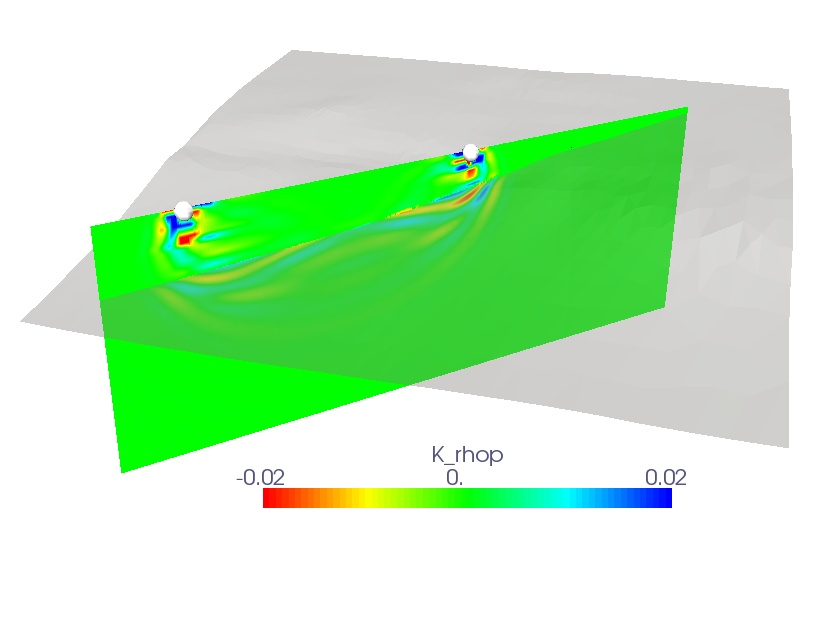
\includegraphics[width=1.\textwidth]{./images/pearl_rhop_kernel.jpg}
\end{center}
\end{minipage}
\end{center}
\caption{Waveform sensitivity to acoustic and elastic structure in a coupled fluid-solid simulation.
The bathymetric surface of the Pearl Harbor model, separating the two media, is shown in gray
together with a vertical cross-section through source (right) and station (left).
Plotted are combined acoustic and elastic kernels using a parameterization (a) $K_\kappa $, $K_\mu$ \& $K_\rho$
and (b) $K_\alpha$, $K_\beta$ \& $K'_{\rho}$.   }
\label{figure:kernelwater}
\end{figure}

\begin{figure}
\begin{center}
\begin{minipage}[t]{0.49\textwidth}
\begin{center}
(a)\\
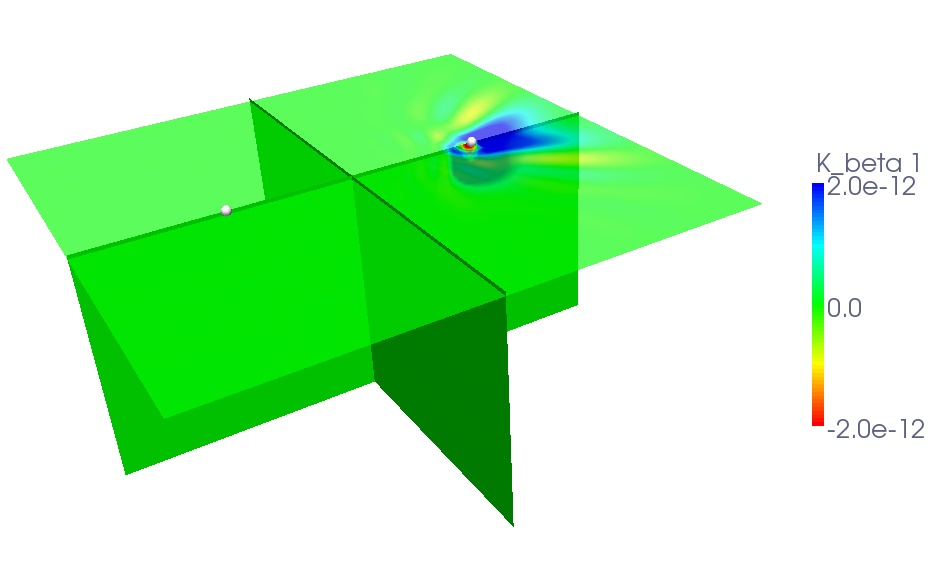
\includegraphics[width=1.\textwidth]{./images/noise_beta_1st.jpg}\\
\end{center}
\end{minipage}
\begin{minipage}[t]{0.49\textwidth}
\begin{center}
(b)\\
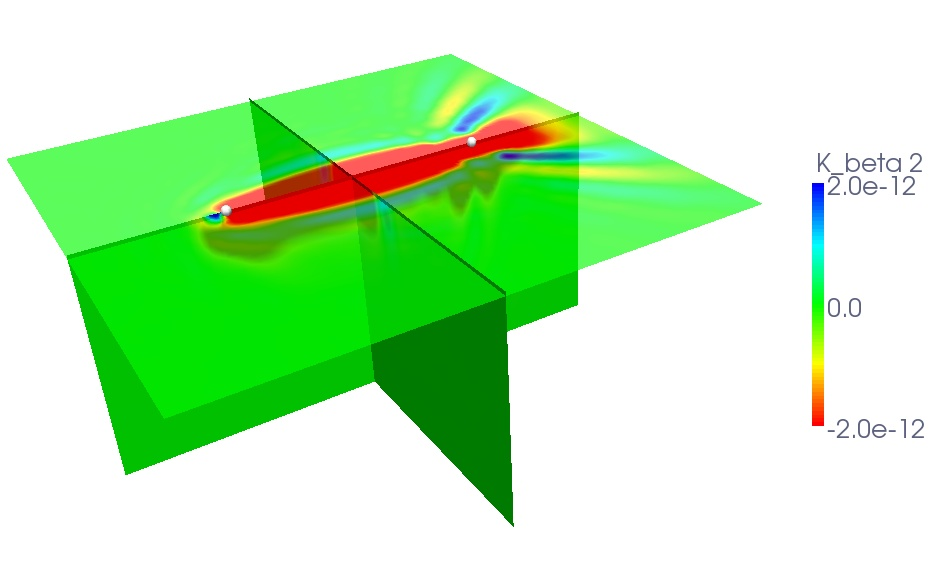
\includegraphics[width=1.\textwidth]{./images/noise_beta_2nd.jpg}\\
\end{center}
\end{minipage}
\begin{minipage}[t]{0.49\textwidth}
\begin{center}
(c)\\
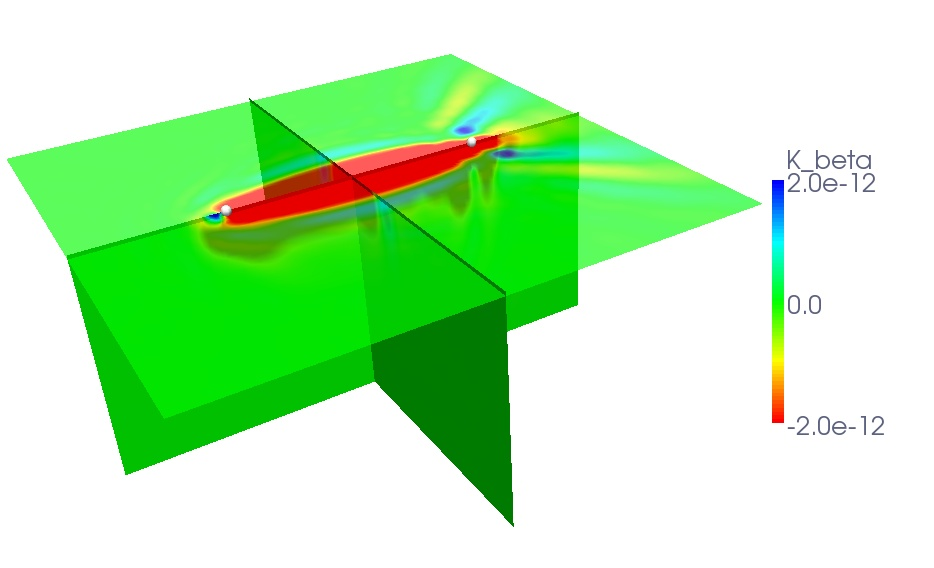
\includegraphics[width=1.\textwidth]{./images/noise_beta_sum.jpg}\\
\end{center}
\end{minipage}
\end{center}
\caption{Noise cross-correlation sensitivity to elastic structure.
Shown are (a) first, (b) second
and (c) summed contributions to the $\langle K_\beta\rangle$ Fr\'echet derivative
in a homogeneous isotropic model.
Plotted are vertical and horizontal cross sections through the line connecting the two receivers (white dots) and perpendicular to this line.
}
\label{figure:kernelnoise}
\end{figure}

\end{document}

